%%%%%%%%%%%%%%%%%%%%%%%%%%%%%%%%%%%%%%%%%%%%%%%%%%%%%%%%%%%%%%%%%%%%%
%% This is a (brief) model paper using the achemso class
%% The document class accepts keyval options, which should include
%% the target journal and optionally the manuscript type. 
%%%%%%%%%%%%%%%%%%%%%%%%%%%%%%%%%%%%%%%%%%%%%%%%%%%%%%%%%%%%%%%%%%%%%
\documentclass[journal=jctcce,manuscript=article]{achemso}

%%%%%%%%%%%%%%%%%%%%%%%%%%%%%%%%%%%%%%%%%%%%%%%%%%%%%%%%%%%%%%%%%%%%%
%% Place any additional packages needed here.  Only include packages
%% which are essential, to avoid problems later. Do NOT use any
%% packages which require e-TeX (for example etoolbox): the e-TeX
%% extensions are not currently available on the ACS conversion
%% servers.
%%%%%%%%%%%%%%%%%%%%%%%%%%%%%%%%%%%%%%%%%%%%%%%%%%%%%%%%%%%%%%%%%%%%%
\usepackage[version=3]{mhchem} 
% Formula subscripts using \ce{}
\usepackage{amsmath}
\usepackage{braket}
\usepackage{color}
% For cross-referencing with SI
\usepackage{xr}
\externaldocument[SI-]{si}

%%%%%%%%%%%%%%%%%%%%%%%%%%%%%%%%%%%%%%%%%%%%%%%%%%%%%%%%%%%%%%%%%%%%%
%% If issues arise when submitting your manuscript, you may want to
%% un-comment the next line.  This provides information on the
%% version of every file you have used.
%%%%%%%%%%%%%%%%%%%%%%%%%%%%%%%%%%%%%%%%%%%%%%%%%%%%%%%%%%%%%%%%%%%%%
%%\listfiles

%%%%%%%%%%%%%%%%%%%%%%%%%%%%%%%%%%%%%%%%%%%%%%%%%%%%%%%%%%%%%%%%%%%%%
%% Place any additional macros here.  Please use \newcommand* where
%% possible, and avoid layout-changing macros (which are not used
%% when typesetting).
%%%%%%%%%%%%%%%%%%%%%%%%%%%%%%%%%%%%%%%%%%%%%%%%%%%%%%%%%%%%%%%%%%%%%
\newcommand*\mycommand[1]{\texttt{\emph{#1}}}



%%%%%%%%%%%%%%%%%%%%%%%%%%%%%%%%%%%%%%%%%%%%%%%%%%%%%%%%%%%%%%%%%%%%%
%% Meta-data block
%% ---------------
%% Each author should be given as a separate \author command.
%%
%% Corresponding authors should have an e-mail given after the author
%% name as an \email command. Phone and fax numbers can be given
%% using \phone and \fax, respectively; this information is optional.
%%
%% The affiliation of authors is given after the authors; each
%% \affiliation command applies to all preceding authors not already
%% assigned an affiliation.
%%
%% The affiliation takes an option argument for the short name.  This
%% will typically be something like "University of Somewhere".
%%
%% The \altaffiliation macro should be used for new address, etc.
%% On the other hand, \alsoaffiliation is used on a per author basis
%% when authors are associated with multiple institutions.
%%%%%%%%%%%%%%%%%%%%%%%%%%%%%%%%%%%%%%%%%%%%%%%%%%%%%%%%%%%%%%%%%%%%%
\author{Marta L{\'o}pez Vidal}
\affiliation[DTU]
{DTU Chemistry - Department of Chemistry, Technical University of Denmark, DK-2800, Kongens Lyngby, Denmark}
\author{Xintian Feng}
\affiliation[UC]{Department of Chemistry, University of California, Berkeley,
California 94720, United States}
\alsoaffiliation{Q-Chem Inc., 6601 Owens Drive, Suite 105 Pleasanton, CA 94588}
%\altaffiliation{Current address: }
\author{Evgeny Epifanovsky}
\affiliation{Q-Chem Inc., 6601 Owens Drive, Suite 105 Pleasanton, CA 94588}
\author{Anna I. Krylov}
%\email{anna.i.krylov@gmail.com}
\affiliation[USC]{Department of Chemistry, University of Southern California, Los Angeles, California 90089-0482}
%\alsoaffiliation[Hamburg]
%{Anna's temporary affiliation in Hamburg?}
\author{Sonia Coriani}
\email{soco@kemi.dtu.dk}
%\phone{+123 (0)123 4445556}
%\fax{+123 (0)123 4445557}
\affiliation[DTU]{DTU Chemistry - Department of Chemistry, Technical University of Denmark, DK-2800, Kongens Lyngby, Denmark}
%%%%%%%%%%%%%%%%%%%%%%%%%%%%%%%%%%%%%%%%%%%%%%%%%%%%%%%%%%%%%%%%%%%%%
%% The document title should be given as usual. Some journals require
%% a running title from the author: this should be supplied as an
%% optional argument to \title.
%%%%%%%%%%%%%%%%%%%%%%%%%%%%%%%%%%%%%%%%%%%%%%%%%%%%%%%%%%%%%%%%%%%%%
\title[CVS-EOM]{A new and efficient equation-of-motion coupled-cluster  
framework for core-excited and core-ionized states}

%%%%%%%%%%%%%%%%%%%%%%%%%%%%%%%%%%%%%%%%%%%%%%%%%%%%%%%%%%%%%%%%%%%%%
%% Some journals require a list of abbreviations or keywords to be
%% supplied. These should be set up here, and will be printed after
%% the title and author information, if needed.
%%%%%%%%%%%%%%%%%%%%%%%%%%%%%%%%%%%%%%%%%%%%%%%%%%%%%%%%%%%%%%%%%%%%%
\abbreviations{NEXAFS}
\keywords{American Chemical Society, \LaTeX}

%%%%%%%%%%%%%%%%%%%%%%%%%%%%%%%%%%%%%%%%%%%%%%%%%%%%%%%%%%%%%%%%%%%%%
%% The manuscript does not need to include \maketitle, which is
%% executed automatically.
%%%%%%%%%%%%%%%%%%%%%%%%%%%%%%%%%%%%%%%%%%%%%%%%%%%%%%%%%%%%%%%%%%%%%
\begin{document}
\begin{center}
\date{\today}
\end{center}
%%%%%%%%%%%%%%%%%%%%%%%%%%%%%%%%%%%%%%%%%%%%%%%%%%%%%%%%%%%%%%%%%%%%%
%% The "tocentry" environment can be used to create an entry for the
%% graphical table of contents. It is given here as some journals
%% require that it is printed as part of the abstract page. It will
%% be automatically moved as appropriate.
%%%%%%%%%%%%%%%%%%%%%%%%%%%%%%%%%%%%%%%%%%%%%%%%%%%%%%%%%%%%%%%%%%%%%
\begin{tocentry}

Some journals require a graphical entry for the Table of Contents.
This should be laid out ``print ready'' so that the sizing of the
text is correct.

Inside the \texttt{tocentry} environment, the font used is Helvetica
8\,pt, as required by \emph{Journal of the American Chemical
Society}.

The surrounding frame is 9\,cm by 3.5\,cm, which is the maximum
permitted for  \emph{Journal of the American Chemical Society}
graphical table of content entries. The box will not resize if the
content is too big: instead it will overflow the edge of the box.

This box and the associated title will always be printed on a
separate page at the end of the document.

\end{tocentry}

%%%%%%%%%%%%%%%%%%%%%%%%%%%%%%%%%%%%%%%%%%%%%%%%%%%%%%%%%%%%%%%%%%%%%
%% The abstract environment will automatically gobble the contents
%% if an abstract is not used by the target journal.
%%%%%%%%%%%%%%%%%%%%%%%%%%%%%%%%%%%%%%%%%%%%%%%%%%%%%%%%%%%%%%%%%%%%%
\begin{abstract}
  We present a fully analytical implementation of the core-valence separation (CVS) scheme for the equation-of-motion (EOM) coupled-cluster singles and doubles (CCSD) method for calculations of core-level states. In the spirit of
the original CVS approximation proposed by Cederbaum, Domcke and Schirmer, pure valence excitations are excluded from the EOM target space and  the frozen-core approximation is imposed on the reference-state amplitudes and multipliers.
This yields an efficient, robust, and accurate EOM-CCSD framework for calculations of excitation and ionization energies as well as state and transition properties (e.g., spectral intensities, natural transition and Dyson orbitals).
The accuracy of the new scheme is improved relative to the results obtained applying the CVS only during the solution of the EOM eigenvalue equations. 
The errors in absolute excitation/ionization energies relative to the experimental reference data are of the order of 0.2--3.0 eV, depending on the K-edge considered and on the basis set used, 
and the shifts are systematic for each edge. 

%RESOLVED.. TEHRE IS A RESIDUAL ERROR
%{\bf I have a question about the shifts that we apply for EOM-EE. I suspect that if we compute EE relative to the corresponding IPs, then we will not need shifts for EE and only for IP. Can we test this quickly?}
%{\bf Sonia: it might not work all the time, as IPs do not always follow , but we can test it}
\end{abstract}

%%%%%%%%%%%%%%%%%%%%%%%%%%%%%%%%%%%%%%%%%%%%%%%%%%%%%%%%%%%%%%%%%%%%%
%% Start the main part of the manuscript here.
%%%%%%%%%%%%%%%%%%%%%%%%%%%%%%%%%%%%%%%%%%%%%%%%%%%%%%%%%%%%%%%%%%%%%
\section{Introduction}

By providing tunable high-energy radiation, advanced light sources
such as X-ray free electron laser (X-FEL) and synchrotron installations enable a variety of X-ray based spectroscopies\cite{Lamberti:XRay:2016,Mobilio:XRay:2014,Bergmann:FEL:17}.
Recent advances in beam quality greatly expanded possible applications of X-rays, giving rise to a proliferation of techniques, including those operating in time-resolved and non-linear regimes \cite{Mobilio:XRay:2014,Lamberti:XRay:2016,Bergmann:FEL:17,Atto:Rev:17,Norman:ChemRev:18}.  
Fundamentally, these spectroscopies exploit electronic transitions involving core orbitals. 
Since core-level binding energies are characteristic of a species, X-ray absorption and X-ray photo-electron spectroscopies (XAS and XPS, respectively) are powerful techniques for probing electronic structure of atoms and molecules~\cite{Stohr1992}.
The localized nature of core orbitals makes X-ray-based spectroscopies sensitive to local environment.  
However, just as in the case of VUV-based techniques\cite{Ahmed:ARPC:16},
theoretical modeling is required to unambiguously assign spectral features and to relate experimental measurements to molecular structures. 
The experimental advances over the past decade have been driving the interest in developing highly accurate theoretical methods for X-ray spectroscopy and, in particular, for time-resolved XAS, which is proving to be a powerful mean to investigate molecular dynamics~\cite{Norman:ChemRev:18,naturecomm,Milne2014,kraus2018}.

Owing to its low computational costs relative to \textit{ab initio} methods, time-dependent (TD) density functional theory (DFT) has been {\color{red}{among the most commonly used techniques}} for modeling absorption spectra\cite{Besley:CoreDFTPersp:10}.
However, TDDFT often fails to deliver an accurate description of spectroscopic properties. Thus, there is an evident need for reliable wave-function-based methods for calculations of XAS spectra. Although more expensive, these methods can be systematically improved, thereby yielding to
results of controlled accuracy\cite{OlsenText}. The focus of this contribution is on coupled-cluster (CC)
approaches~\cite{koch1990,Stanton:93:EOMCC,Christiansen_IJQC,krylov_eom_2008,WF_Properties_Review,CC_EOMCC_Bartlett,Christiansen2006,Christiansen:EOMRev:11}, which are among the most successful \textit{ab initio} methods for molecular properties 
{\color{red}{and electronic spectra in the UV-vis region}}, 
{\color{red}{to describe}}  absorption and ionization phenomena {\color{red}{in the X-ray spectral region}}\cite{coriani2012jctc,Peng2015,coriani2012pra,coriani2015jcp,naturecomm}.

Although ionization or excitations of core electrons superficially appear to be similar to valence transitions, the numerical experiments have shown that direct application of
standard approaches to core-level transitions leads to unsatisfactory results\cite{Norman:ChemRev:18}, due to the following essential features of core-ionized and core-excited states. 
First, these states have open-shell character\cite{Krylov:OSRev}.
Second, the core-level states lie very high in energy (hundreds of electron volts, depending on the edge).
Third, orbital relaxation effects are much more important
for core states than for valence states because the outer orbitals are more delocalized and better shielded from the nuclear charge than the tight and localized core orbitals.
Fourth, these transitions appear to be much more sensitive to the effect of the
environment\cite{Sadybekov:CoreIE:17,Kongsted:DECore:18}.
Fifth, these high-lying states are metastable with respect to electron 
ejection\cite{Reinhardt:CS:1982,KrylovResReview}, i.e., they are Feshbach resonances that can autoionize via two-electron transitions
in which one valence electron fills the core hole and a second valence electron is ejected.
Thus, they are embedded in the ionization continuum and their description within Hermitian quantum
mechanics is problematic. 

Multistate methods, such as EOM-CC \cite{Emrich:81:EOM1,koch1990,Stanton:93:EOMCC,Christiansen2006,krylov_eom_2008,Christiansen:EOMRev:11,CC_EOMCC_Bartlett}, can effectively describe multiconfigurational wavefunctions, tackle open-shell character and  orbital relaxation effects in one computational scheme. The effect of the environment can be included by using a variety of implicit or explicit solvent models. 
However, dealing with high-energy interior states,
especially with those embedded in autodetaching continuum, is more problematic.  
Although the Davidson procedure can be modified
to solve for the eigenstates dominated by the desired transition (MOM-like\cite{Gill:MOM:08}) or
lying within the desired energy range\cite{Zuev:Solvers:14,Peng2015},
the convergence and numeric stability are strongly affected by the presence of the continuum.
An attempt to compute such states often produces pseudo-continuum states in which one electron occupies the most diffuse orbital\cite{Zuev:PYP:10}. Because in Hermitian quantum mechanics, the resonances are not represented by a single state, but rather by an increased density of states in the continuum\cite{Moiseyev:Book:11}, 
the representation of resonances in a discretized continuum is inherently prone to numeric instabilities.
Although the EOM-CC methods can describe resonances by using complex-scaled and
CAP-augmented approaches\cite{KrylovResReview},
such calculations are much more expensive than regular bound-state
calculations. Here we focus on alternative, less expensive approximate
methods for modeling spectroscopic properties of the core-level states.

Our strategy for tackling issues due to the continuum nature of the core levels is based on employing the core-valence separation (CVS) approximation proposed by \citeauthor{Cederbaum1980}
in 1980~\cite{Cederbaum1980}. By decoupling the core excitations  from the rest of the configurational space, 
the CVS allows one to extend standard methods for excited and ionized states to the core-level states\cite{wenzel2014,wenzel2015,coriani2015jcp}.
Effectively, CVS results in decoupling of the highly excited core states from the continuum of valence excitations; it also leads to a significant reduction of the computational costs.
The core states can also be decoupled from the continuum by excluding double excitations 
from the configurational space and treating them perturbatively\cite{Sadybekov:CoreIE:17}. 
Although numerically stable,
this approach suffers from insufficient description of orbital relaxation\cite{Sadybekov:CoreIE:17}.
Because the CVS approximation admits selected double excitations that are crucial for describing orbital relaxation, 
CVS-EOM/LR-CCSDs\cite{coriani2015jcp} yields negligible decline in accuracy, as compared 
to full EOM-CCSD/LR-CCSD results~\cite{coriani2012pra,coriani2012jctc,fransson2013jcp}.

An implementation of the CVS within EOM-CC and Linear Response (CCLR) theories has been reported by \citeauthor{coriani2015jcp}\cite{coriani2015jcp}. In this work, the CVS was deployed as an {\em{a posteriori}} projection applied at each iteration of the solution of the EOM/CCLR equations to eliminate excitations that do not involve at least one core electron, 
whereas the ground state amplitudes and Lagrangian multipliers retained all possible types of excitations.  
Here, a different strategy is presented: the zero-order wave-function parameters are computed within the frozen-core (fc) approximation and the subsequent EOM/CCLR equations are solved analytically imposing the core-valence separation. 
The respective state and transition properties such as oscillator strengths, natural transition orbitals (NTOs), Dyson orbitals, exciton descriptors, and so on are obtained from the appropriate densities between different target-state manifolds. Specifically, transition properties  
can be computed between the ground state and the core-excited state, as well as between a valence-excited and a core-excited state. 
This yields an efficient scheme for simulating, e.g., near-edge absorption fine structure (NEXAFS) spectra of both ground and excited states. The latter is required to simulate UV-pump/X-ray-probe experiments and to obtain core-ionization potentials and Dyson orbitals for XPS spectra of medium size molecules.
We report illustrative results for NEXAFS and core IEs
of all K-edges in neon, water, ammonia, ethylene, vinylfluoride, ozone, adenine, as well as the transient (time-resolved) NEXAFS spectrum of uracil.

\section{Theory}

\subsection{EOM-CCSD}
In the EOM-CC approach, the target-state wave functions are parameterized using the following ansatz:~\cite{sekino1984linear,Stanton:93:EOMCC,CC_EOMCC_Bartlett,krylov_eom_2008}
\begin{equation}
\langle \Psi_L | = \langle \Phi_0 |{L}e^{-T}~~;
%\end{equation}
%\begin{equation}
\quad \quad \quad | \Psi_R \rangle =  e^{T} {R}| \Phi_0 \rangle 
\end{equation}
where $| \Phi_0 \rangle $ is a reference Slater determinant and \textit{T}, \textit{R} and $L^\dagger$ are excitation operators.\\
The excitation operator \textit{T} is the cluster operator:\cite{Note-1}
\begin{equation}
\begin{aligned}
T &= \sum_{\mu} t_{\mu} \tau_{\mu} = T_1 + T_2 + \dots + T_N \\
T_1 &= \sum_{ia} t_i^a a_a^{\dagger}a_i ,\hspace{0.3cm}  T_2 = \frac{1}{4}\sum_{ijab} t_{ij}^{ab} a_a^{\dagger}a_i a_b^{\dagger}a_j ,\hspace{0.3cm}\dots 
\end{aligned}
\end{equation}
with $\tau_{\mu}$ being the excitation operator and $t_{\mu}$ the corresponding cluster amplitudes determined by the CC equations for the reference state:
\begin{equation}
\langle \Phi_\mu | \bar{H} - E_\text{CC} | \Phi_0 \rangle = 0~~; 
\qquad\qquad E_\text{CC} = \langle \Phi_0| \bar{H} | \Phi_0 \rangle
\end{equation}
where $\langle \Phi_\mu |$'s represent $\mu$-tuple excited determinants and $\bar{H}$ is the similarity transformed Hamiltonian:
\begin{equation}
\bar{H} = e^{-T} H e^{T}.
\end{equation}
The operator $R$ is a general excitation operator:
  \begin{equation}
   R = R_0 + R_1 + \dots + R_n \equiv \sum_\mu r_\mu \tau_\mu
   \end{equation}
and $L$ is a de-excitation operator:
  \begin{equation}
   L = L_0 + L_1 + \dots + L_n \equiv \sum_\mu l_\mu \tau^\dagger_\mu
   \end{equation}
  The choice of the reference state and the exact form of $R$ and $L$ depend on the EOM method to be used\cite{krylov_eom_2008,CC_EOMCC_Bartlett}.
  Furthermore, in practical calculations the excitation {\color{red}{and de-excitation}} operators must be truncated to some tractable level of excitation. 
In this work, we focus on the EOM-CCSD family of methods in which
the cluster operator $T$ is truncated to single (S) and double (D) excitations, and so are the excitation $R$ and de-excitation $L$ operators.

One of the most obvious applications of EOM theory is the calculation of electronically excited states\cite{sekino1984linear,Stanton:93:EOMCC}. In this approach, referred to as EOM-EE (EOM for excitation energies), the optimal reference state is usually the closed-shell ground-state Hartree-Fock determinant and the $R$ and $L$ operators conserve the number of electrons and their spin, taking the following forms:
{\color{red}{
\begin{equation}
R^\text{EE}= \sum_{ia} r_i^a a_a^\dagger a_i + \frac{1}{4} \sum_{ijab} r_{ij}^{ab} a_a^\dagger a_i a_b^\dagger a_j + \dots
\end{equation}
\begin{equation}
L^\text{EE}= \sum_{ia} l_i^a a_i^\dagger a_a + \frac{1}{4} \sum_{ijab} l_{ij}^{ab} a_i^\dagger a_a a_j^\dagger a_b + \dots
\end{equation}
}}
Another common use of EOM is calculations of ionization energies by the EOM-IP (EOM for ionization potentials)
method\cite{Stanton:94:AnlDer,Stanton:EOMRev:03,PAP:EOMIP}. In this case, the excitation operator changes the number of electrons in the system, assuming the 
following from:
\begin{equation}
R^\text{IP}= \sum_{i} r_i a_i + \frac{1}{4} \sum_{ija} r_{ij}^{a} a_a^\dagger  a_j a_i + \dots
\end{equation}

The EOM amplitudes $r_\mu$ and $l_\mu$ are found as stationary points of the EOM functional:
\begin{equation}
E = \frac{\langle \Psi_L| H | \Psi_R \rangle}{\langle \Psi_L | \Psi_R \rangle} 
\end{equation}
By applying the bi-variational principle~\cite{Bivariational_Lowdin,levchenko2004equation}, one arrives  
to the non-symmetric eigenvalue problem:
\begin{equation}
\langle \Phi_\mu | \bar{H} - E | R \Phi_0 \rangle = 0~~; 
\qquad\qquad
\langle \Phi_0 L | \bar{H} - E | \Phi_\mu \rangle = 0, 
\end{equation}
where the eigenvectors of the Hamiltonian are chosen to form a biorthogonal set\cite{Stanton:93:EOMCC}: 
\begin{equation}
\langle \Phi_0 L_i| R_j \Phi_0 \rangle = \delta_{ij}
\end{equation}

Thus, the implementation of EOM-CCSD method boils down to the diagonalization of the effective Hamiltonian $\bar{H}$ in the basis of the reference and of singly and doubly excited determinants, which can be written in matrix form as:
\begin{equation}
\label{Hbar}
\bar{H} = 
\begin{pmatrix}
E_{CC} & \bar{H}_{OS} & \bar{H}_{OD} \\
0 & \bar{H}_{SS} & \bar{H}_{SD} \\
0 & \bar{H}_{DS} & \bar{H}_{DD} \\
\end{pmatrix}
\end{equation}
giving rise to the EOM-CCSD right and left eigenvalue equations:
\begin{equation}
\label{righteq}
\begin{pmatrix}
\bar{H}_{SS} - E_{CC} & \bar{H}_{SD} \\
\bar{H}_{DS} & \bar{H}_{DD} - E_{CC} \\
\end{pmatrix}
\begin{pmatrix}
R_1 \\
R_2 \\
\end{pmatrix} 
= \omega 
\begin{pmatrix}
R_1 \\
R_2 \\
\end{pmatrix}
\end{equation}

\begin{equation}
\label{lefteq}
\begin{pmatrix}
L_1 & L_2 \\
\end{pmatrix} 
\begin{pmatrix}
\bar{H}_{SS} - E_{CC} & \bar{H}_{SD} \\
\bar{H}_{DS} & \bar{H}_{DD} - E_{CC} \\
\end{pmatrix}
= \omega
\begin{pmatrix}
L_1 & L_2 \\
\end{pmatrix}
\end{equation}
where $\omega$ is the energy difference with respect to the reference state.

In practice, Eqs.~\eqref{righteq} and \eqref{lefteq} are solved iteratively using a generalized Davidson's iterative diagonalization procedure\cite{Davidson,hirao1982generalization,rettrup1982iterative} which requires the computation of the right $\sigma$ and left $\tilde{\sigma}$ trial vectors:
\begin{equation} 
\sigma_1 = ([\bar{H}_{SS}-E_{CC}]R_1)_1 + (\bar{H}_{SD}R_2)_1
\end{equation}
\begin{equation} 
\sigma_2 = (\bar{H}_{DS}R_1)_2 + ([\bar{H}_{DD}-E_{CC}]R_2)_2
\end{equation}

\begin{equation} 
\tilde{\sigma}_1 = (L_1[\bar{H}_{SS}-E_{CC}])_1 + (L_2\bar{H}_{DS})_1
\end{equation}
\begin{equation} 
\tilde{\sigma}_2 = (L_1\bar{H}_{SD})_2 + ([L_2\bar{H}_{DD}-E_{CC}])_2
\end{equation}
{\color{red}{
In EOM-CC, molecular properties are traditionally calculated as expectation values, using one-particle density matrices like
\begin{equation}
\label{gamma}
 \gamma_{pq} = \langle \Psi_L | a_p^\dagger a_q | \Psi_R \rangle~.
\end{equation}
}}
%It should be stressed that properties calculated as expectation values do not include relaxation effects.
%{\color{blue}{SONIA: what do you mean by this? Are you talking about orbital relaxation (not included in EOM nor in Response), or something else?}}
%
In the present study, we focus on transition properties involving core states, specifically, the oscillator strengths $f$ between the ground state and the core-excited states, and between valence-excited and core-excited states. 
These can be formulated via contractions of property integral matrices and transition density matrices, for instance,
\begin{equation}
f (i \to j) = \frac{2}{3}(\omega_j - \omega_i) \sum_{\alpha=x,y,z} \mu^{i\to j}_{\alpha} 
\mu^{j\to i}_{\alpha}
\end{equation}
where 
\begin{equation}
\mu_\alpha^{i\to j}
= \sum_{pq} \mu^{\alpha}_{pq} \gamma^{ i\to j}_{pq}~; \quad \quad
\mu_\alpha^{j\to i} = \sum_{rs} \mu^{\alpha}_{rs} \gamma^{j\to i }_{rs}
% \end{aligned}
\label{strength}
\end{equation}
Above, $\mu^\alpha$ refers to a specific Cartesian component of the electric dipole operator and the state $i$ can be either the ground state and an excited state.


The transition density matrices $\gamma^{i\to j}_{pq}$ and $\gamma^{j\to i}_{pq}$ are generalizations of Eq.~\eqref{gamma}, and their specific form in the fc-CVS-EOM-CCSD framework is discussed in the next sections.
{\color{red}{We remind the reader that the EOM transition densities differ from those derived within (non-linear) coupled cluster response theory as they do not contain non-linear terms, that can be viewed as originating from the amplitudes' relaxation to the external perturbation. Moreover, orbital relaxation is also omitted, as traditionally done within coupled cluster response theory.~\cite{Christiansen_IJQC} }}
Transition density matrices describe  the changes in electron density upon excitation and 
can be interpreted as exciton wavefunction\cite{Luzanov:TDM-1:76,Luzanov:DMRev:12,Plasser2012,Plasser2014}
when expressed in coordinate space:
\begin{equation}
\chi(r_p,r_h) = \sum_{pq} \gamma_{pq} \phi_p(r_p) \phi_q(r_h),
\end{equation}
where $r_p$ and $r_h$ denote particle (electron) and hole coordinates,
respectively (using $r_h=r_p=r$, $\chi$ is reduced to the transition density).  
Properties of the exciton can be quantified by various expectation
values, i.e., exciton size, hole-particle separation and correlation, and so on.
These exciton descriptors help to assign state characters\cite{Plasser2012,Plasser2014,Plasser2014:1}.
Applying a singular value decomposition (SVD) to the transition matrices yields the so-called NTOs~\cite{Martin2003,Plasser2012,Plasser2014,Plasser2014:1,Bappler2014,Mewes2018}, which can be used to
describe the electronic excitations in terms of hole-particle excitons:
\begin{equation}
\chi(r_p,r_h) = \sum_K \sigma_K  \tilde{\phi}^p_K(r_p) \tilde{\phi}^h_K(r_h),
\end{equation}
where $\tilde \phi^p_K$ and $\tilde \phi^h_K$ are particle and hole orbitals obtained by SVD 
of $\gamma$ and $\sigma_K$  
are the corresponding  singular values. Usually, only a few
$\sigma_K$ are non-zero, giving rise to simple interpretation of excited-state characters
in terms of one-electron excitations. Note that the sum of $\sigma_K^2$ is equal to the squared norm of $\gamma$, which provides a simple metric quantifying the single-electron character of the transition, i.e., for pure single excitations, $||\gamma||$=1. 

\subsection{The fc-CVS-EOM-CCSD method}
{\color{red}Different flavors of separation between core and valence excitations have been realized for a variety of approximate wavefunction methods as well as for TDDFT, and we refer the interested reader to Ref.~\citenum{Norman:ChemRev:18} 
for a recent overview. 

In the CVS-CC framework of Ref.~\citenum{coriani2015jcp}, for example, an effective core-valence separation was introduced (as a projection) in the solution of the CC eigenvalue equations since, physically, the core-excited states are energetically far away from the valence excited states.

Already in 1980, \citeauthor{Cederbaum1980}~\cite{Cederbaum1980} suggested that,
since core orbitals are strongly localized in space and energetically are well separated from the valence orbitals, one can 
%The CVS approximation~\cite{Cederbaum1980,Barth1985} 
%exploit this fundamental feature to 
one can decouple core and valence orbitals by zeroing out the respective blocks of the model Hamiltonian, such that the solutions of the Schr\"odinger equation can be separated into core and valence domains.
In 1985, \citeauthor{Barth1985}\cite{Barth1985}  
implemented this idea within the second-order 
algebraic diagrammatic construction method ADC(2)~\cite{Schirmer,Dreuw:ADCrev:2014}
by observing that, in view of negligible coupling between core and valence orbitals, all the following two-electron Coulomb integrals are negligible

\begin{align}
\label{screening}
\langle Ip|qr \rangle = \langle pI|qr \rangle = \langle pq|Ir \rangle =
\langle pq|rI \rangle \approx 0 \\\nonumber 
\langle IJ | pq \rangle = \langle pq |IJ \rangle \approx 0 \\\nonumber
\langle IJ | Kp \rangle = \langle IJ | pK \rangle = 
\langle Ip | JK \rangle = \langle pI | JK \rangle \approx 0
\end{align}
where small letters indicate general valence orbitals, and capital letters  core orbitals. As a consequence,
one can omit the blocks of the ADC propagator matrix ${\bf M}$ involving these integrals and therefore decouple pure valence excitations from excitations involving core electrons. 
This idea was later extended to all other members of the ADC family of propagator methods~\cite{Schirmer2000,Dreuw:ADCrev:2014,wenzel2014} [AND FORM THE BASIS FOR THE TDDFT SCHEMES??].
}
%following the original work of~\citeauthor{Barth1985}\cite{Barth1985}},
Since MP2 is an underlying wave-function for the ADC propagator\cite{Dreuw:ADCrev:2014}, omitting the integrals in Eq.~\eqref{screening} immediately corresponds to using the frozen-core approximation for the MP2 ground state energy.

{\color{red}{Similarly, 
it can be straightforwardly shown that, if the above-mentioned  criterion of negligible Coulomb integrals is used within the CCSD ansatz in the canonical basis,~\cite{Purvis_and_Bartlett} 
the resulting CCSD energy and the amplitude equations for the ``valence-only'' 
amplitudes $t^a_{i}$ and $t^{ab}_{ij}$
are identical to those obtained adopting the frozen-core 
approximation -- that is,
assuming that all ground-state amplitudes and multipliers where at least one occupied index refer to a core orbital are zero.
%on the 
%{\color{red}{ground-state CC parameters}}
%CC wave-function, as it can be easily verified 
%, i.e. by restricting the occupied indices in the cluster operator $T$ (and corresponding amplitudes) to valence occupied orbitals.
%{\color{red}{}}

Thus, in the here-proposed fc-CVS-EOM-CCSD method, we use the frozen core approximation during the determination of the ground-state amplitudes $t_\mu$ and Lagrangian multipliers ${\lambda}_{\mu}$ and, at the same time, impose that the excitation/ionization operators $R$ and $L$ involve at least one core orbital. 
This introduces restrictions on the left and right EOM equations, and on the density matrices used to obtain the molecular properties.  
}}
%We refer to the resulting approach as fc-CVS-EOM-CCSD method.

The programmable expressions for obtaining the right and left excitation vectors within the fc-CVS-EOM-CCSD methods have been derived from Ref.~\citenum{levchenko2004equation} and for the density matrices from Ref.~\citenum{levchenko2005analytic} and can be found in the Supplementary Information.\\
As an illustrative example, we show below how the expression of the right linearly transformed vector elements $\sigma_i^a$ is modified for the fc-CVS case. The general expression for  
$\sigma_i^a$ is\cite{levchenko2004equation}
\begin{equation}
\label{sigma_ia}
        \sigma_i^a = \sum_b F_{ab} r_i^b -
            \sum_j F_{ij} r_j^a -
            \sum_{jb} I^{1}_{ibja} r_{j}^{b} +
            \sum_{jb} F_{jb} r_{ij}^{ab} -
            \frac{1}{2} \sum_{jkb} I^{6}_{jkib} r_{jk}^{ab} -
            \frac{1}{2} \sum_{jbc} I^{7}_{jabc} r_{ij}^{bc}
\end{equation}
with 
\begin{flalign}
\label{original}
&F_{ia} = f_{ia} + \sum_{jb} t_j^b \langle ij ||ab \rangle   & \notag \\
&F_{ij} = f_{ij} + \sum_{a} t_i^a f_{ja} 
                + \sum_{ka} t_k^a \langle jk ||ia \rangle
                + \sum_{kab} t_i^a t_k^b \langle jk ||ab \rangle
                + \frac{1}{2} \sum_{kbc} t_{jk}^{ac} \langle jk ||bc \rangle  & \notag \\
&F_{ab} = f_{ab} - \sum_{i} t_i^a f_{ja} 
                - \sum_{ic} t_i^c \langle ia ||bc \rangle
                + \sum_{ijc} t_i^c t_j^a \langle ij || bc \rangle
                - \frac{1}{2} \sum_{jkc} t_{jk}^{ac} \langle jk ||bc \rangle  &  \\
&I^1_{iajb} = \langle ia ||jb \rangle 
				- \sum_k t_k^b \langle jk||ia \rangle 
                - \sum_c t_{i}^c \langle jb||ac \rangle 
                + \sum_{kc} t_{i}^c t_k^b \langle jk||ac \rangle 
                - \sum_{kc} t_{ik}^{bc} \langle jk||ac \rangle   & \notag \\
&I^6_{ijka} =
            \langle ij || ka \rangle -
            \sum_c t_{k}^c \langle ij || ac \rangle   & \notag \\
&        I^7_{iabc} =
            \langle ia || bc \rangle -
            \sum_j t_j^a \langle ij || bc \rangle   & \notag
\end{flalign}
It is convenient to further split the occupied orbitals $(i,j,k,l,\ldots)$ into the two sub-blocks: occupied valence 
{\color{red}{labelled with an additional $v$ subindex, $(i_v,j_v,k_v,l_v,\ldots)$}}, and
occupied core orbitals denoted by a capital letter {\color{red}{$(I,J,K,L,\ldots)$}} .
As anticipated, the CVS approximation is implemented by:
{\color{red}{$(i)$}} reducing the set of occupied orbitals to 
only the core ones in the excitation process and,
{\color{red}{$(ii)$}} freezing the core orbitals in 
optimization of the ground state {\color{red}{CC wavefunction parameters (amplitudes and multipliers).}}
Hence, by restricting the EOM excitations to core excitations only, all terms involving {\color{red}{only}} 
valence excitations disappear in the equations above. 
The frozen-core approximation further simplifies the equations since 
the {\color{red}{terms in Eqs.~\eqref{original}}} involving ground-state amplitudes vanish for the core orbitals,
{\color{red}{or, in other words, only ground state amplitudes %and multipliers 
with valence occupied orbitals are retained in the fc-CVS case}}.

The fc-CVS expression for {\color{red}{the linearly transformed trial vector in Eq.~\eqref{sigma_ia}}} 
thus reads as follows:
{\color{red}{
\begin{equation} 
\begin{aligned}
\sigma_I^a 
=& \sum_{b} F_{ab} r_I^b 
- \sum_{J} F_{IJ} r_J^a 
- \sum_{Jb} I^1_{IbJa} r_J^b
+ \sum_{Jb} F_{Jb} r^{ab}_{IJ} 
+ \sum_{j_vb} F_{j_vb} r^{ab}_{Ij_v} \\
&- \sum_{Jk_vb} \langle Jk_v || Ib \rangle r^{ab}_{Jk_v}
- \frac{1}{2} \sum_{JKb} \langle JK || Ib \rangle r^{ab}_{JK}
- \frac{1}{2} \sum_{Jbc} I^7_{Jabc} r^{bc}_{IJ} 
- \frac{1}{2} \sum_{j_vbc} I^7_{j_vabc} r^{bc}_{Ij_v} 
\end{aligned}
\end{equation}
%
with
%
\begin{flalign}
&F_{Ia} = f_{Ia} + \sum_{j_vb} t_{j_v}^b \langle Ij ||ab \rangle   & \notag \\
&F_{IJ} = f_{IJ} + \sum_{k_va} t_{k_v}^a \langle J{k_v} ||Ia \rangle    & \notag \\
&F_{i_v a} = f_{i_v a} + \sum_{j_vb} t_{j_v}^b \langle i_vj_v ||ab \rangle   & \\
&I^1_{IaJb} = \langle Ia ||Jb \rangle - \sum_{k_v} t_{k_v}^b \langle J{k_v}||Ia \rangle    & \notag  \\
&I^7_{Iabc} =
            \langle Ia || bc \rangle -
            \sum_{j_v} t_{j_v}^a \langle I{j_v} || bc \rangle   & \notag
\end{flalign}
}}
The same strategy has been followed for the derivation of the other linearly transformed vector blocks, as for the expressions of the (transition) density matrices, 
reported in the Supplementary Information.
{\color{red}{We underline that the integral screening in 
Eq.~\eqref{screening} has only been used to justify the use of the frozen-core approximation in the determination of the ground-state CC 
wavefunction parameters, whereas terms containing such integrals have been 
retained in the determination of the target states' energies and transition properties. Even if they can be expected to be small, they might increase 
the flexibility of our method to address core-relaxation effects via correlation.}}

{\color{red}{To conclude this session, it is appropriate to discuss whether the
fc-CVS-EOM-CCSD method still yields size-intensive excited state energies.
As discussed, for instance, in Refs.~\cite{Stanton:95:PT-EOMCC,wang:2014:EOMCCSOC},
size-intensivity of the excitation energies is guaranteed if the first column of the
matrix representation of the effective Hamiltonian $\bar{H}$ is as given in Eq.~\eqref{Hbar}.
Beside the $E_{CC}$ energy, this column contains the terms 
$\langle \Phi_\mu | \exp(-T) H \exp(T) | \Phi_0 \rangle$, 
where $|\mu \rangle$ is,
for CCSD, either a single or a double-excitation determinant with respect to the reference Slater determinant $|\Phi_0\rangle$, see Eqs.~\eqref{amplitudes}.  

In our case, the $\langle \Phi_{i_v}^{a} | \exp(-T) H \exp(T) | \Phi_0 \rangle$ and
$\langle \Phi_{i_v j_v}^{ab} | \exp(-T) H \exp(T) | \Phi_0 \rangle$ elements are zero,
since they correspond to the (frozen-core) solution of the amplitude equations.
The remaining terms, where the occupied indices are either a core $I$, a core $J$ or 
both, are trivially zero, since we adopt the frozen-core approximation. 
}}

\section{Computational details}
We implemented the fc-CVS-EOM-CC method in the Q-Chem electronic structure package~\cite{qchem_feature,Qchem_MP_paper} using
the libtensor library\cite{libtensor_paper}.
The geometries of \ce{H2O}, \ce{NH3}, \ce{CO}, \ce{C2H4}, \ce{C2H3F} and \ce{O3} were optimized at the {\color{red}{fc-}}CCSD(T)/cc-pVQZ level using CFOUR~\cite{cfour}. For 9H-adenine, we considered 
both planar and non-planar structures taken from the literature. The non-planar one was optimized at the {\color{red}{fc-}}RI-MP2/cc-pVTZ level~\cite{SarahMCD2018}, whereas the planar one was optimized at the B3LYP/cc-pVTZ level.~\cite{Santoro2014}
For the TR-NEXAFS simulations on uracil, we used different structures: an optimized MP2/cc-pVTZ ground-state structure, a ground-state structure and an S$_1$ {\color{red}{minimum}} 
both optimized at the SF-BH\&HLYP/6-31+G(d,p) level from Ref.~\citenum{uracil_herbert}, and two stationary-point (i.e., zero-gradient)
structures for the S$_1$ and S$_2$ excited states
obtained at the EOM-CCSD/aug-cc-pVDZ level of theory. 
All structures were planar or almost planar.
%{\color{red}{Neither the S$_1$ nor the S$_2$ EOM structures are minima.}}

Depending on the system, we considered different basis sets  in the (TR-)NEXAFS calculations:  Pople's 6-311++G** (pure $d$ functions), Dunning's aug-cc-pVDZ, aug-cc-pVTZ and aug-cc-pCVTZ sets. In selected cases, the basis sets were further augmented with uncontracted Rydberg-type functions whose exponents were computed according to the prescription of \citeauthor{Rydberg_basis}\cite{Rydberg_basis} 
Experimental data were taken from:  Ref.~\citenum{nexafs_thymine_adenine}
for adenine, Ref.~\citenum{Neon_exp} for Neon,
Ref.~\citenum{NEXAFS_H2O_NH3_CH4_Exp} for \ce{H2O} and \ce{NH3},
Ref.~\citenum{NEXAFS_CO_C_Exp} and~\citenum{NEXAFS_CO_O_Exp} for \ce{CO},
Ref.~\citenum{NEXAFS_C2H4_CH2CHF_Exp} for \ce{C2H4} and \ce{C2H3F} and Ref.~\citenum{ozone_nexafs_xps} for \ce{O3}.
The experimental NEXAFS spectrum of uracil is from Ref.~\citenum{nexafs_cytosine_uracil}.
All experimental spectra were digitized from the 
original references using WebPlotDigitizer~\cite{WPD}. 
The spectra were generated using a Python script and NTOs were visualized using MOLDEN~\cite{molden}.

\section{Results and discussion}
\subsection{Near-Edge Absorption Spectroscopy and core ionization energies}

To test the performance of our method, we first considered the neon atom.  Table~\ref{SI-Tab:Neon} reports the computed excitation energies and IEs with three different basis sets, all supplemented with Rydberg-type functions (with $n$=2.5--4.5); the corresponding spectra are shown in Fig.~\ref{fgr:neon}. 
As the atomic NEXAFS spectra are due to transitions from the 1$s$ orbital to Rydberg states, the inclusion of Rydberg-type functions (or, alternative, a large set of diffuse functions) is mandatory in order to reproduce the Rydberg progression of peaks in the experimental spectrum.~\cite{coriani2012pra}

The NEXAFS spectra have been shifted, along with the IEs, to align with the first peak of the experimental NEXAFS spectrum (estimated to be at 867.10~eV). After the shift, the computed peaks match the  experimental ones almost perfectly. Of the three sets, Dunning's aug-cc-pCVTZ (+Rydberg) yields the smallest absolute shift from experiment (+0.19 eV), followed by -0.43 eV of the aug-cc-pVTZ (+Rydberg) set, versus -0.84 eV of Pople's  6-311+G**(+Rydberg). The spectral profiles in the two Dunning sets overlap completely after the alignment. 

With respect to previously reported CCSD results~\cite{coriani2012pra} obtained in the aug-cc-pCVTZ(+Rydberg) basis using the Lanczos algorithm with all electrons correlated (i.e., no CVS), the absolute shift from experiment in the fc-CVS-EOM-CCSD method is lower and has an opposite sign ($+$0.19 eV versus $-$1.07 eV). The shift is also smaller than that obtained 
in the CVS approach of Ref.~\citenum{coriani2015jcp}. 

\begin{figure}[H]
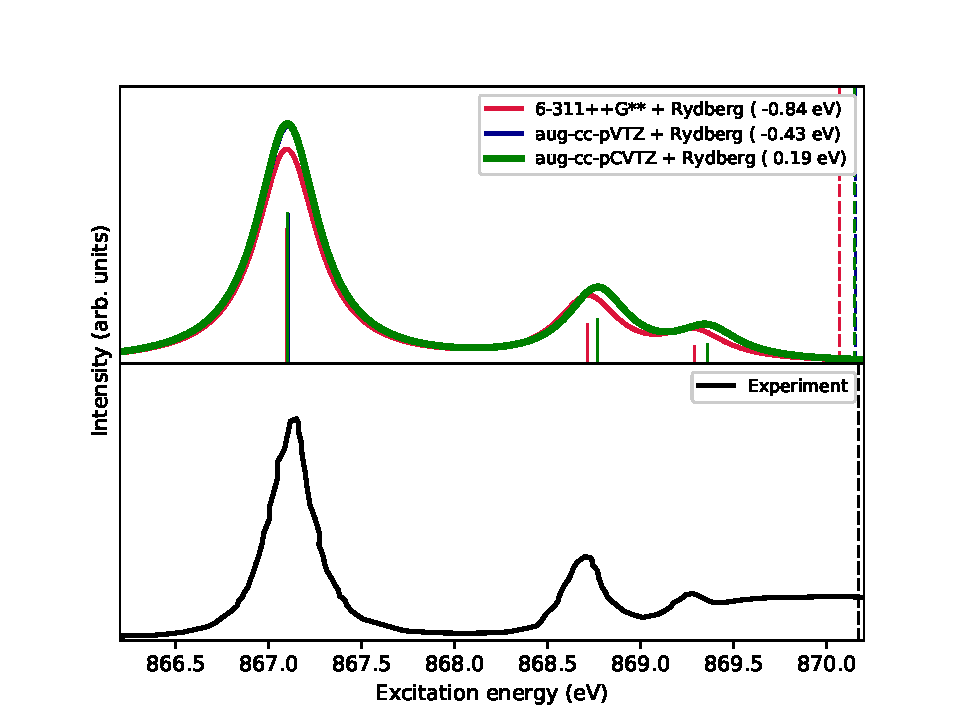
\includegraphics[width=0.9\textwidth]{Spectra/Ne_aCT.pdf}  
\caption{Neon. fc-CVS-EOMEE-CCSD X-ray absorption spectra obtained by convolution of the computed excitation energies and oscillator strengths with a Lorentzian function (FWHM = 0.4 eV). The experimental spectrum was digitized from Ref.~\citenum{Neon_exp}. 
The vertical dashed lines correspond to the core ionization energies. The experimental IE is 870.17 eV. 
The energy shifts 
required to align the NEXAFS profiles in each basis set with the
experimental one are indicated in parenthesis. The computed IEs have been shifted by the same amount as used to align the NEXAFS profiles.
\label{fgr:neon}
}
\end{figure}

The NEXAFS and IE values of \ce{H2O} are reported in Table~\ref{SI-Tab:Water}, with the corresponding spectra shown in Fig.~\ref{fgr:water}. The upper panel of Fig.~\ref{fgr:water} shows the spectra for the chosen basis sets without Rydberg-type functions, whereas the middle panel shows those obtained including the Rydberg-type functions.
Besides an overall shift (taking the value 534.0 eV as reference for the experimental first peak maximum, which varies slightly for the three bases, the separation between the two first peaks is practically the same, whereas huge differences are observed for the other bands, which are known to be of partial Rydberg character.
Both relative intensity and position of the third band and the following ones are strongly overestimated in the bases without Rydberg functions. 
In this case, the energy shifts required to realign with the experimental spectrum are also smaller than those used in 
the LR-CVS calculation from Ref.~\citenum{coriani2015jcp}  and in the full-space Lanczos calculation from Ref.~\citenum{coriani2012pra}.
Remarkably, in the aug-cc-pCVTZ basis the shift is smaller that in the aug-cc-pVTZ basis, whereas the reverse trend has been observed using the LR-CVS approach of Ref.~\citenum{coriani2015jcp}. Thus, the current approach shows a systematic improvement of the results with respect to the basis set increase.

\begin{figure}[H]
  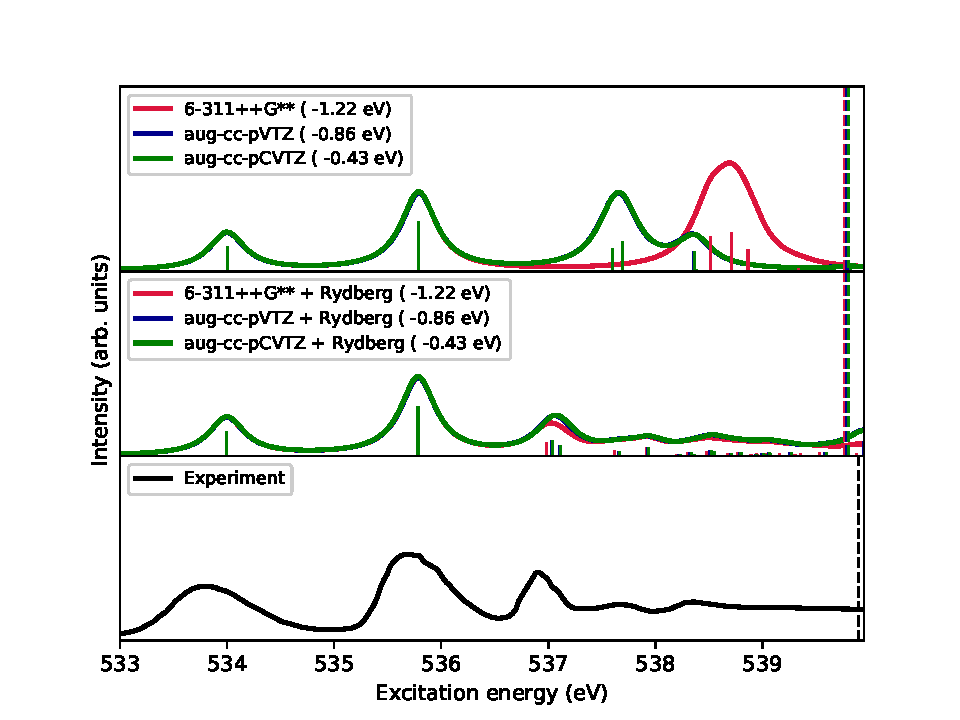
\includegraphics[width=0.9\textwidth]{Spectra/H2O.pdf}
  \caption{Water. fc-CVS-EOMEE-CCSD O-edge X-ray absorption spectra  obtained by convolution of the spectral data in Table~\ref{SI-Tab:Water} with a Lorentzian function (FWHM = 0.4 eV). The experimental spectrum was digitized from Ref.~\citenum{NEXAFS_H2O_NH3_CH4_Exp}. \label{fgr:water}
Dashed vertical lines correspond to the IEs. The energy shifts 
required to align the NEXAFS profiles in each basis set with the
experimental one are indicated in parenthesis.
The computed IEs have been shifted by the same amount as used to align the NEXAFS profiles.}
\end{figure}

%%%%%%%%%%%%%%%%%%%%%%%%  AMMONIA 

Another system whose gas-phase NEXAFS is dominated by Rydberg states is \ce{NH3}. Fig.~\ref{fgr:ammonia} shows
the computed spectra; the raw data are 
in Table~\ref{SI-Tab:Ammonia}. The spectra were aligned with respect to the peak maximum of the first experimental band, estimated at 400.53 eV. As for the previous systems, the Dunning basis shows a smaller shift compared to the experimental peaks ($-$0.68 eV vs $-$1.04 eV). Neither Pople's 6-311++G** nor Dunning's aug-cc-pVTZ can correctly reproduce the third and higher bands without inclusion of the Rydberg-type functions. 

\begin{figure}[H]
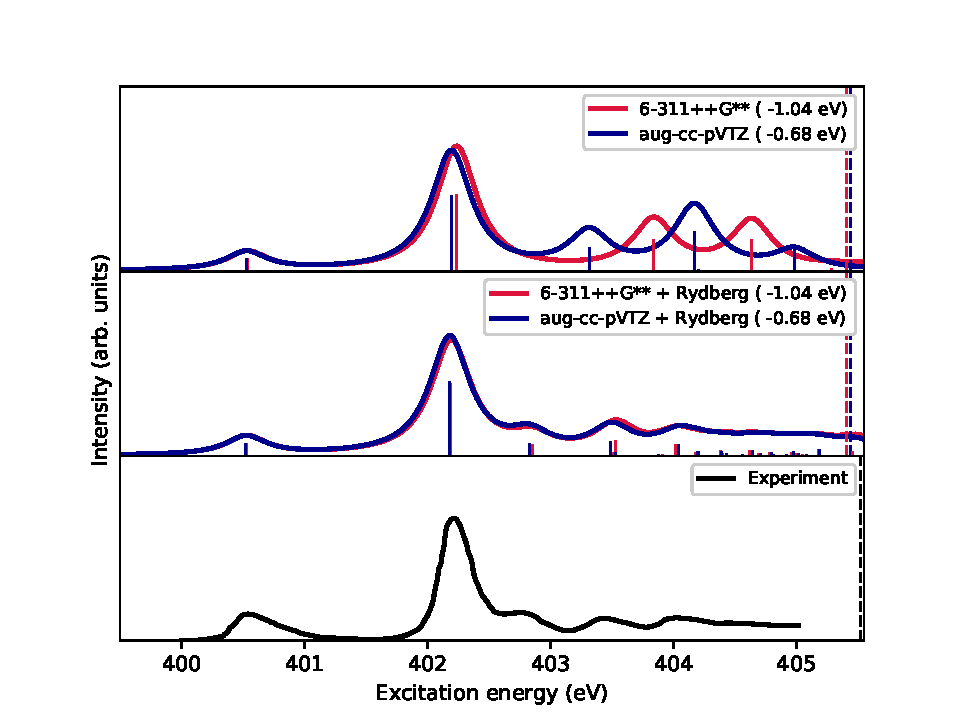
\includegraphics[width=1\textwidth]{Spectra/NH3.pdf}
\caption{Ammonia. fc-CVS-EOMEE-CCSD N-edge X-ray absorption spectra obtained from convolution of the spectral data in Table~\ref{SI-Tab:Ammonia} 
with a Lorentzian function (FWHM = 0.4 eV). The experimental spectrum was digitized from Ref.~\citenum{NEXAFS_H2O_NH3_CH4_Exp}. Dashed vertical lines indicate the IEs.\label{fgr:ammonia}.
The energy shifts 
required to align the NEXAFS profiles in each basis set with the
experimental one are indicated in parenthesis. The computed IEs have been shifted by the same amount as used to align the NEXAFS profiles.}
\end{figure}

%%%%%%%%%%%%%%%%%%%%%%%%  CARBON MONOXIDE
%Experimental data: 287.4 eV [43] and 534.2 eV [44],
Table~\ref{SI-Tab:CO} presents the spectral data for C and O edges of carbon monoxide and the corresponding spectra are shown in Fig.~\ref{fgr:co_both}. The two upper panels in the figure show the main NEXAFS bands, experimentally observed 
in between 286.5 and 289.0 eV for carbon and in between 533 and 537 eV for oxygen. The middle and bottom panels of Fig.~\ref{fgr:co_both}
show the (much weaker) peaks observed at higher frequencies below 
the ionization limit.

The position of the dominant C-edge 1$s\to \pi^\ast$ band  is overestimated by 0.50 eV in the 6-311++G** + Rydberg basis set,
and underestimated by 0.05 eV in the aug-cc-pVTZ + Rydberg basis. 
The O-edge 1$s\to \pi^\ast$ band is overestimated by about 1.16 eV in Pople's set, and by 0.66 eV in Dunning's basis. The additional features of the main experimental bands are due to the vibronic progression, which is not included in our calculations. 

Upon alignment of the computed spectra with the main peak of the experimental ones, the Rydberg transitions are still slightly misaligned, see mid panels of Fig.~\ref{fgr:co_both}.
Nonetheless, all weaker 3$s\sigma$, 3$p\pi$, 3$p\sigma$, 3$d\pi$, 4$s\sigma$, and 4$s\pi$ transitions can be identified in the computed spectra of each edge, thought once again without their finer vibronic progressions. The assignments can be verified by realignment of the first peak of the first progression, as shown in the bottom panels of Fig.~\ref{fgr:co_both}. 

%{\color{red}{After alignment with respect to the energy of the main NEXAFS peak, the computed IPs are still slightly overestimated.}}

\begin{figure}\vspace{-0.5cm}
\begin{tabular}{cc}
%Shifted respect to first experimental peak estimated at 287.3 eV
\hspace{-1cm}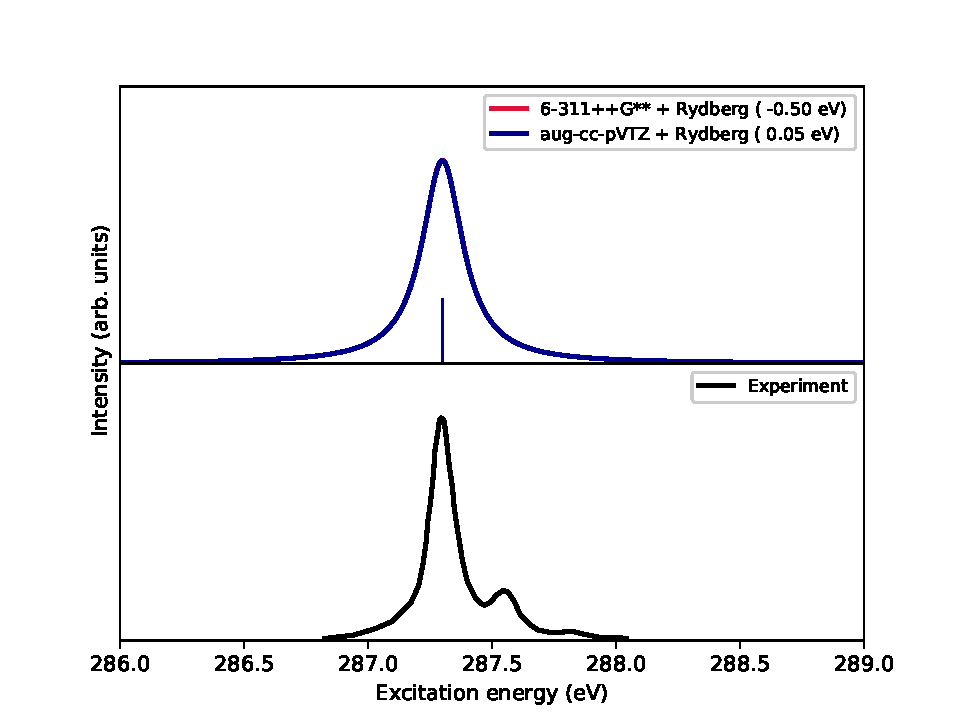
\includegraphics[width=0.50\textwidth]{Spectra/CO_C_1.pdf} &
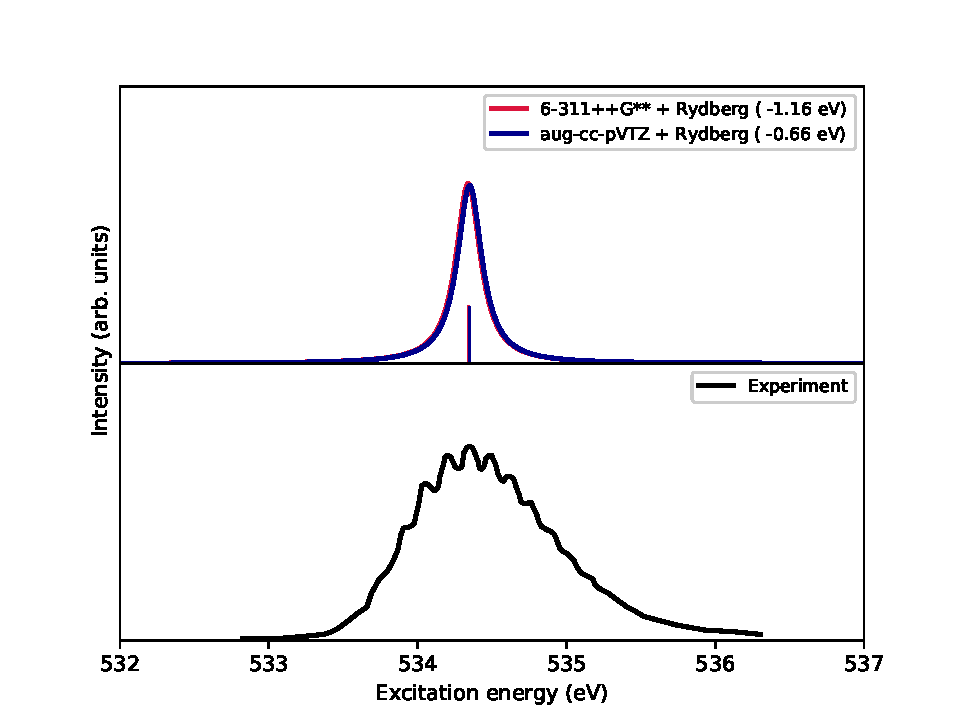
\includegraphics[width=0.50\textwidth]{Spectra/CO_O_1.pdf}\\\vspace{-0.5cm}
%SONIA: I think this was the wrong one
%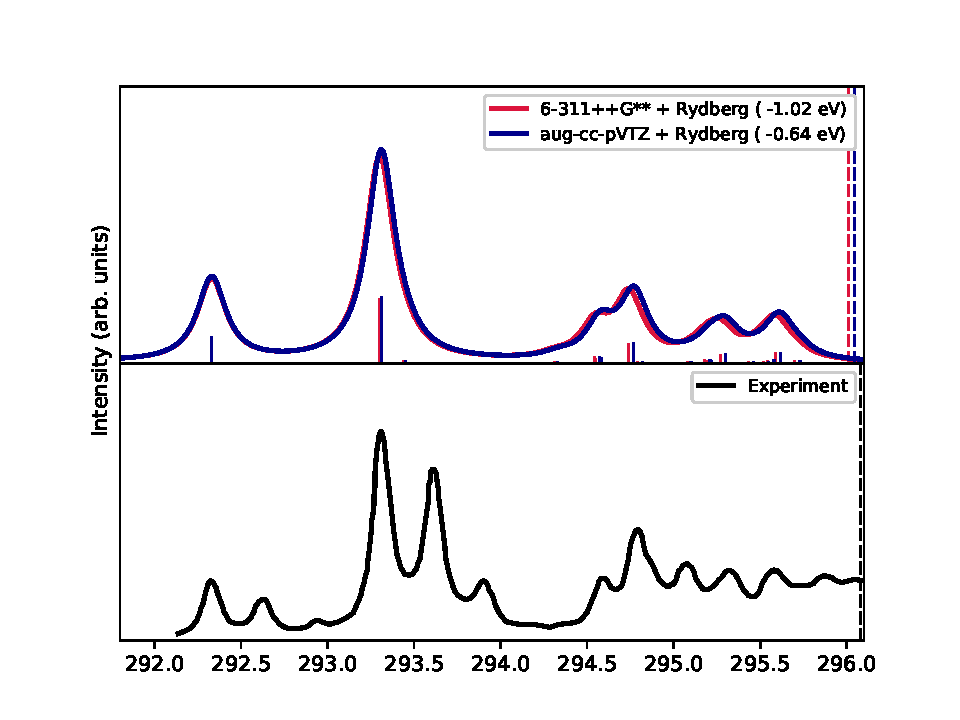
\includegraphics[width=0.55\textwidth]{Spectra/CO_C_2.pdf} & 
\hspace{-1cm}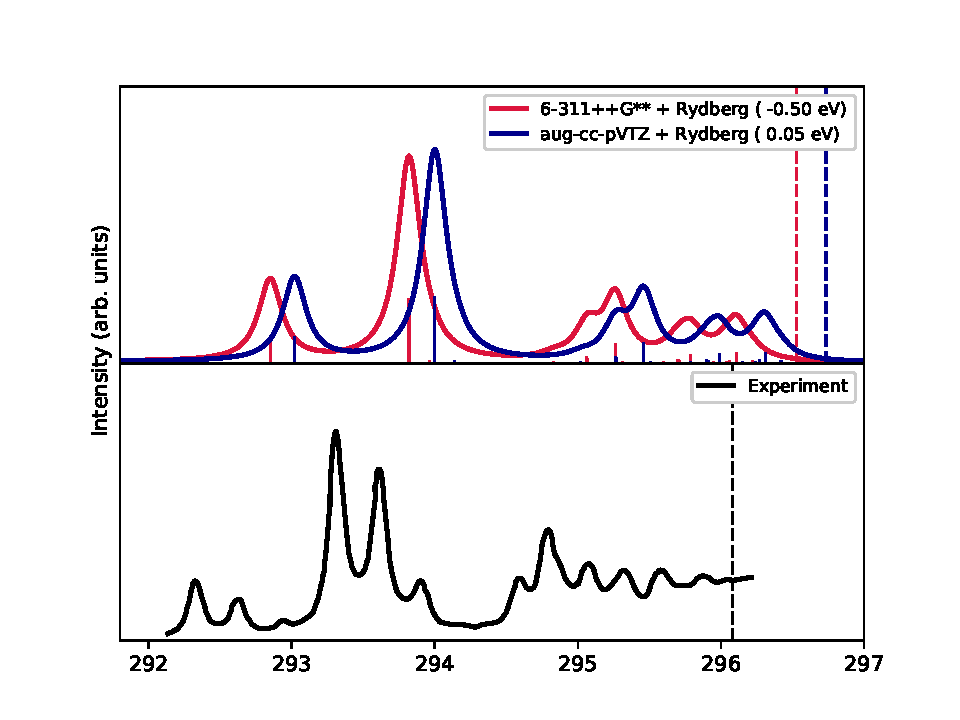
\includegraphics[width=0.50\textwidth]{Spectra/CO_C_2_newshift.pdf} &
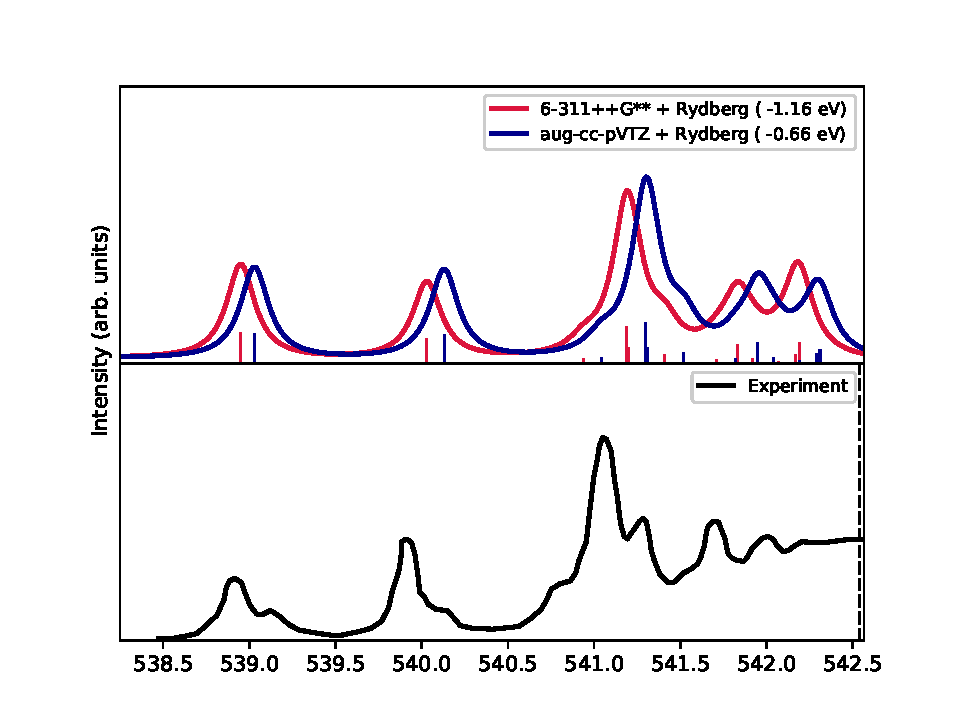
\includegraphics[width=0.50\textwidth]{Spectra/CO_O_2.pdf} \\\vspace{-0.5cm}
%Shifted respect to second experimental peak estimated at 292.33 eV
\hspace{-1cm}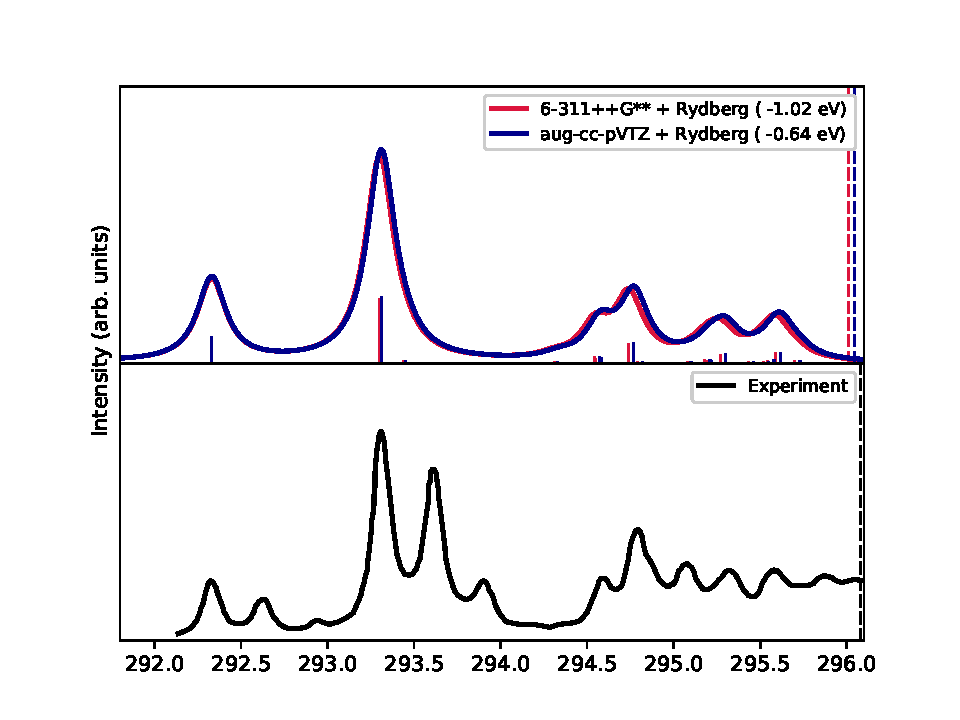
\includegraphics[width=0.50\textwidth]{Spectra/CO_C_2.pdf} &
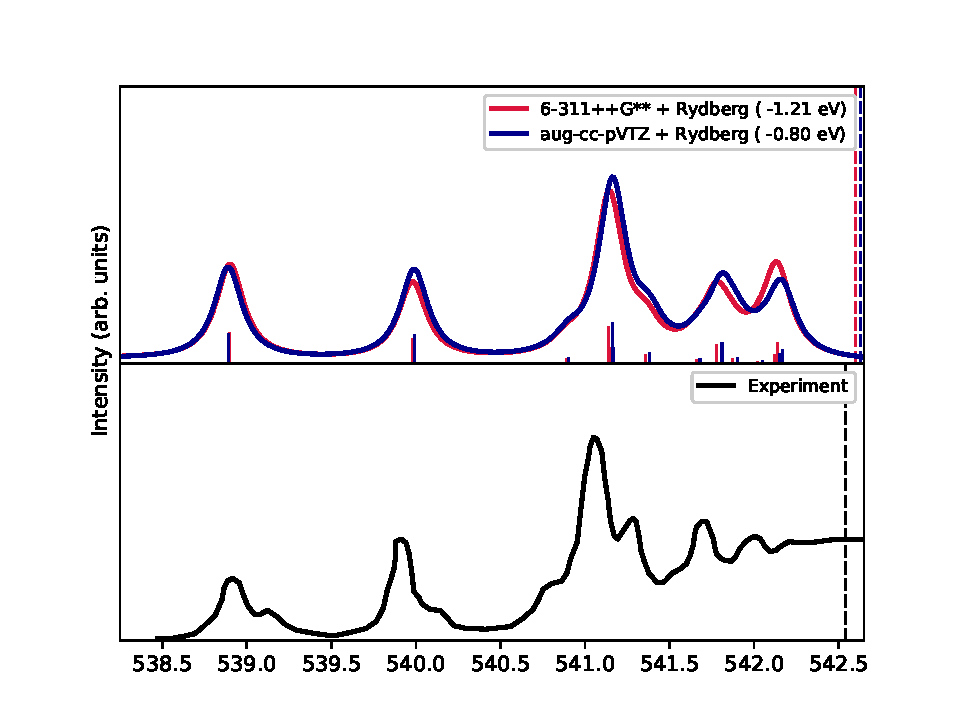
\includegraphics[width=0.50\textwidth]{Spectra/CO_O_2_newshift.pdf}\\
%  %Shifted respect to first experimental peak estimated at 534.35 eV
%  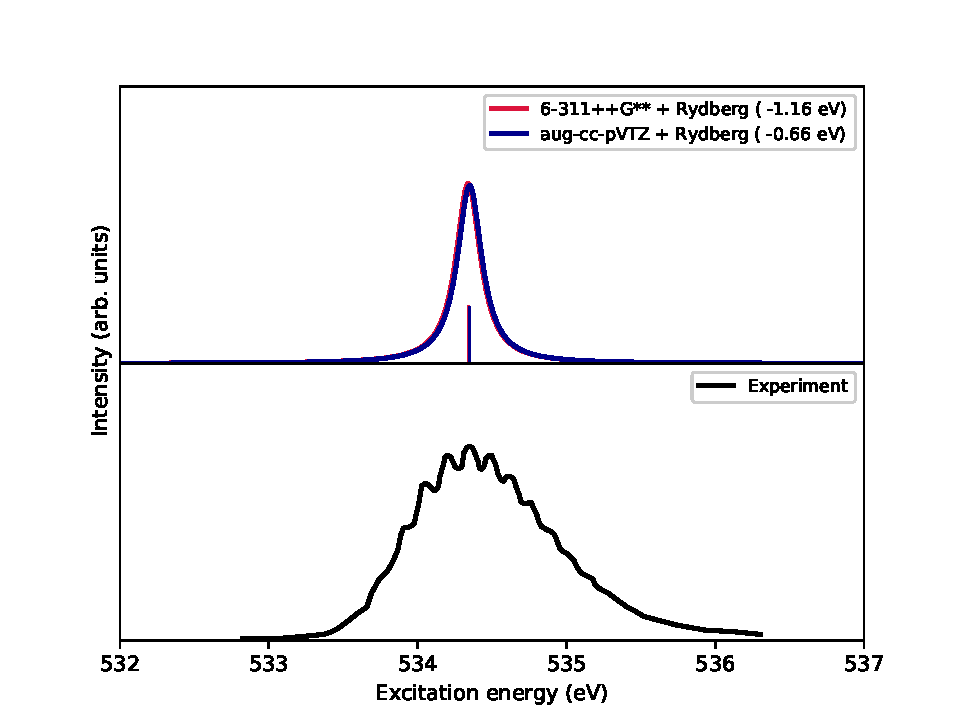
\includegraphics[width=0.42\textwidth]{Spectra/CO_O_1.pdf}
%  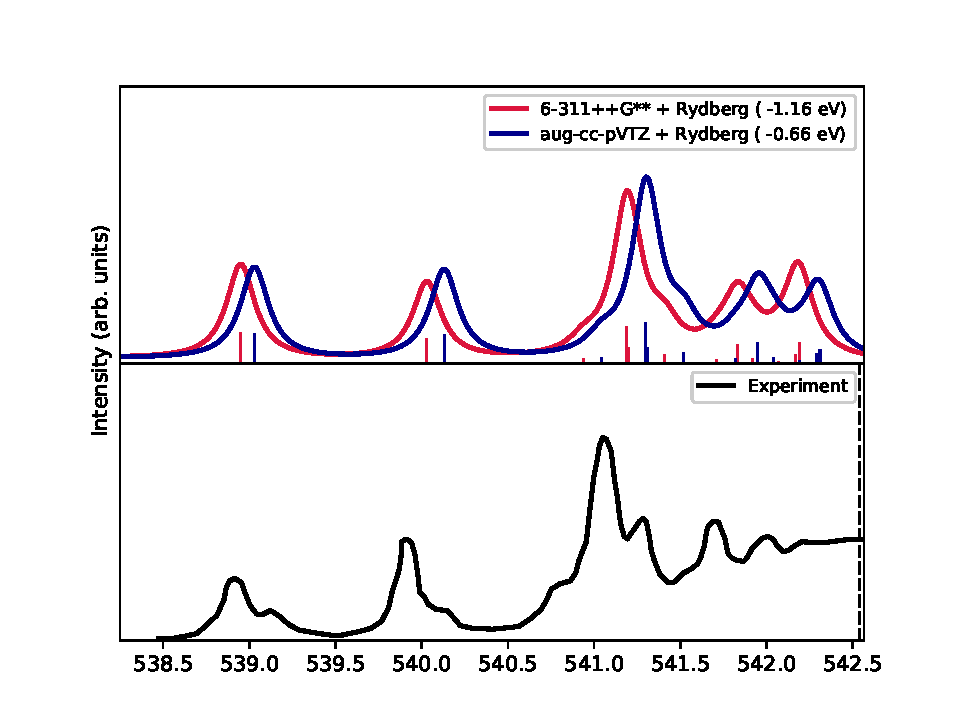
\includegraphics[width=0.42\textwidth]{Spectra/CO_O_2.pdf}
%
%  %Shifted respect to second experimental peak estimated at 538.90 eV
%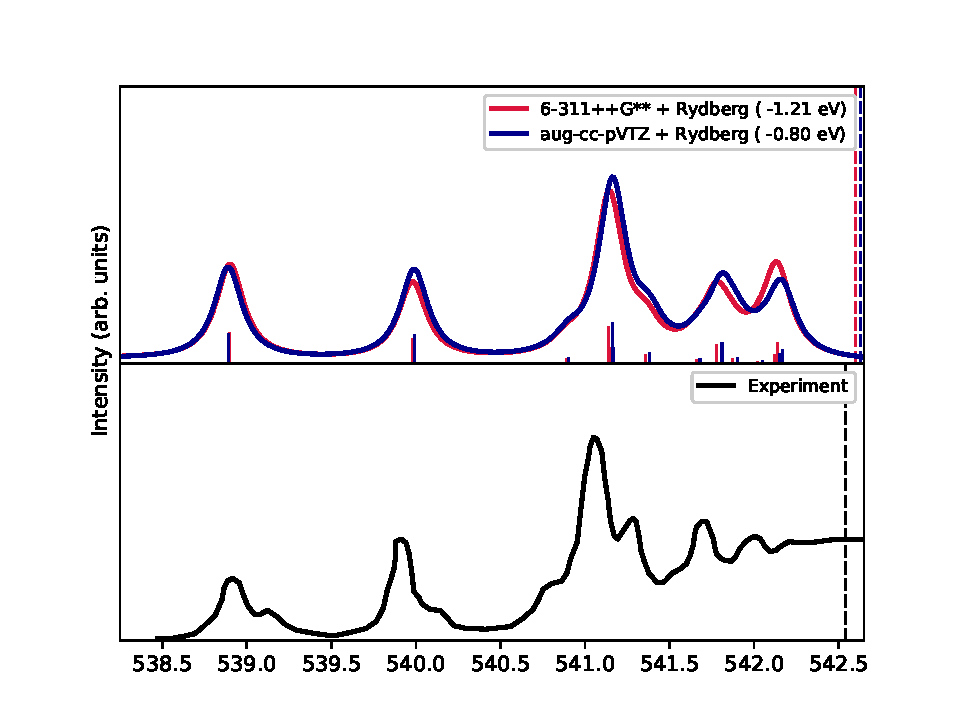
\includegraphics[width=0.42\textwidth]{Spectra/CO_O_2_newshift.pdf}
\\C K-edge & O K-edge
\end{tabular}
\caption{Carbon monoxide. fc-CVS-EOMEE-CCSD
C K-edge (left) and O K-edge (right) X-ray absorption spectra, obtained by convolution of the computed excitation energies and oscillator strengths with a Lorentzian function (FWHM = 0.2 eV).
The upper panels show the main 1$s\to\pi^\ast$ band,
the mid and bottom panels the band progressions of the weaker 1$s\to$ 3$s\sigma$, 3$p\pi$, 3$d\pi$, 4$s\sigma$, and 4$s\pi$ transitions.
The experimental spectra were digitized from Ref.~\citenum{NEXAFS_CO_C_Exp}.
Vertical dashed lines correspond to the IEs.
\label{fgr:co_both}
}
\end{figure}

%%%%%%%%%%%%%%%%%%%%%%% ETHENE %%%%%%%%%%%%%%%%%%%%%%%%%%%%%%%%%
 %Shifted respect to first experimental peak estimated at 284.65 eV
\clearpage
Fig.~\ref{fgr:ethylene} reports the computed spectra of ethylene
obtained by convolution of the spectral data in Table~\ref{SI-Tab:Ethylene}. In this case, the Rydberg functions also improve the description of the higher energy region approaching the ionization limit (third experimental band~\cite{NEXAFS_C2H4_CH2CHF_Exp}). 
The second band in the experimental spectrum corresponds to three excitations in the computed spectra.
%{\bf{do we want to elaborate on this?}}.
The overall shift is 0.44 eV in the aug-cc-pVTZ(+Rydberg) set and 0.90 eV for Pople's 6-311++G**(+Rydberg) set. Upon realignment
with respect to the 1$s\to \pi^\ast$ absorption energy, the IE obtained with Pople's set is slightly underestimated compared to the experimental IEs.

\begin{figure}
  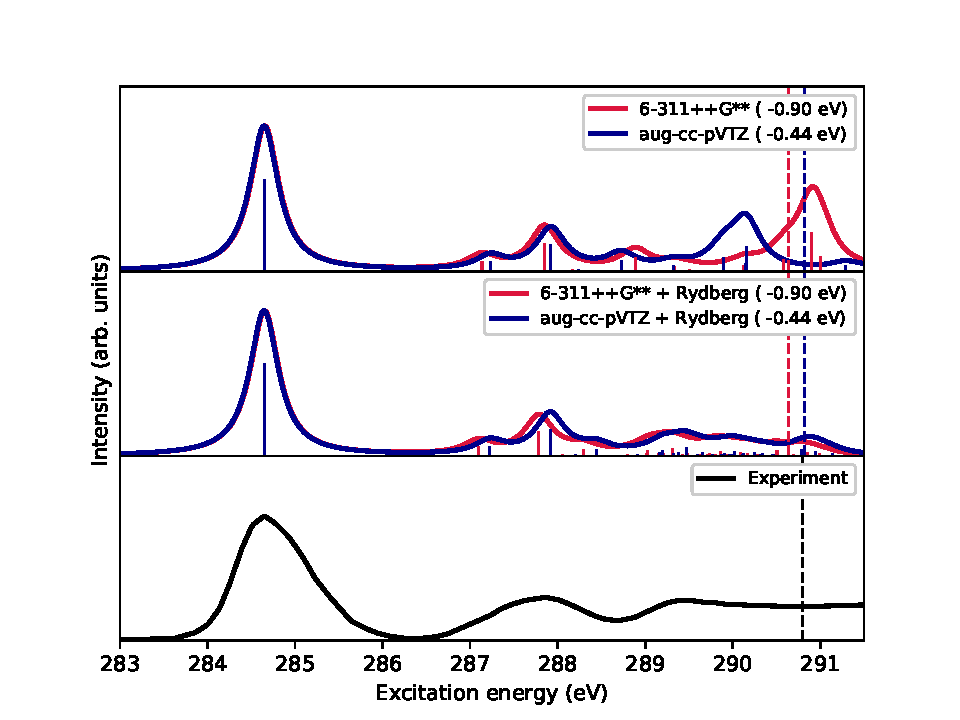
\includegraphics[width=0.9\textwidth]{Spectra/C2H4.pdf}
  \caption{Ethylene. fc-CVS-EOMEE-CCSD X-ray absorption spectra by  Lorentzian broadening (FWHM = 0.4 eV) of the computed excitation energies and oscillator strengths. The  experimental spectrum was digitized from Ref.~\citenum{NEXAFS_C2H4_CH2CHF_Exp}. The vertical dashed lines correspond to the IEs.
The energy shifts 
required to align the NEXAFS profiles in each basis set with the
experimental one are indicated in parenthesis. The computed IEs have been shifted by the same amount as used to align the NEXAFS profiles.
\label{fgr:ethylene}}
\end{figure}



%%%%%%%%%%%%%%%  VINYLFLUORIDE %%%%%%%%%%%%%%%%%%%%%%%%%%%%%
Fig.~\ref{fgr:vinylfluoride:C} shows the computed X-ray spectra 
at the C edge in vinylfluoride (\ce{CH2CHF}); the raw data are given in Table~\ref{SI-Tab:Vinylfluoride:C}.
The computed spectra were shifted to align them to the first experimental peak~\cite{NEXAFS_C2H4_CH2CHF_Exp}, whose position we estimated to be at 285 eV. The applied shift is $-0.44$ eV
for Dunning's set, and $-0.91$ eV for Pople's set. 
Inclusion of Rydberg-type functions in the basis set has a more 
modest effect than in the case of ethylene.
NTOs of the most intense core excitations obtained with the
6-311++G** basis set are shown in Table~\ref{vinylfluoride-ntos-Cedge}, 
allowing us to identify from which of the two C atoms they originate from and the character of the transition. 

The X-ray absorption spectra obtained at the fluorine edge of \ce{CH2CHF} are shown in Fig.~\ref{fgr:vinylfluoride:F}; the raw data are given in Table~\ref{SI-Tab:Vinylfluoride:F}.
In the experimental spectrum, digitized from Ref.~\citenum{NEXAFS_C2H4_CH2CHF_Exp}, only two peaks are clearly
discernible, with absolute energies assigned at (689.2$\pm$2.0) eV 
and 690.6$\pm$2.0 eV (1$s_F\to \sigma^*$ (C-F)).
In the experimental study, the first peak is assigned to a 
1$s_F \to \pi^*$(C=C) transition, and the second one to
a 1$s_F\to \sigma^*$ (C-F) transition. Inspection of 
our results in Table~\ref{SI-Tab:Vinylfluoride:F} and of the NTOs
in Table~\ref{NTOs:fluorine} indicates that 
the first band results from two almost degenerate transitions, 
1$s_F\to \sigma^*$ (C--F) and 1$s_F \to \pi^*$(C=C). The third excitation (second experimental band)
also appears to be of 1$s_F\to \sigma^*$ (C-F) character.


The experimental IE is at 693.26 eV~\cite{jolly1984core}.
The computed spectra in the Pople set (with and without Rydberg functions) are realigned by $-1.98$ eV, and those for the Dunning basis by $-1.58$ eV. 

%Shifted respect to first experimental peak estimated at 285 eV
\begin{figure}[H]
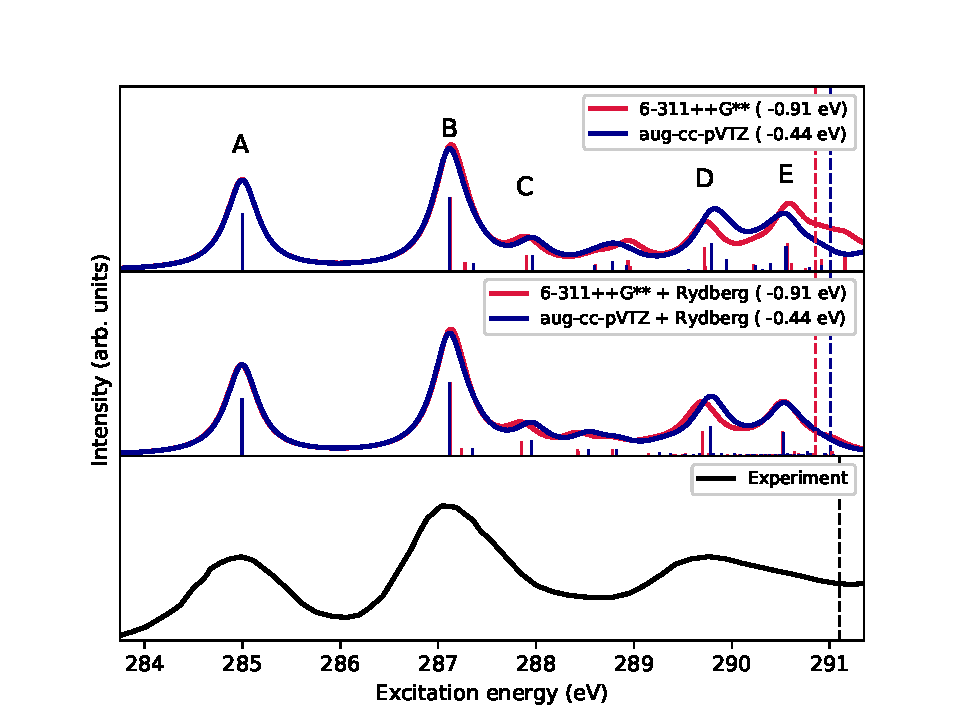
\includegraphics[width=0.9\textwidth]{Spectra/CH2CHF.pdf}  
\caption{Vinyl fluoride. fc-CVS-EOMEE-CCSD X-ray absorption spectra at the C-edge obtained by convolution of the computed energies and oscillator strengths with a Lorentzian function (FWHM = 0.4 eV). The experimental spectrum was digitized from Ref.~\citenum{NEXAFS_C2H4_CH2CHF_Exp}. The dashed vertical lines correspond to the 
IEs of the 1$s$ electron on the carbon atom of the \ce{CH2} group. The IEs of the 1$s$ electron of C$_{\ce{CHF}}$ atom are outside the displayed frequency range
(experimental IE 293.48 eV).
The energy shifts 
required to align the NEXAFS profiles in each basis set with the
experimental one are indicated in parenthesis. The computed IEs have been shifted by the same amount as used to align the NEXAFS profiles.
\label{fgr:vinylfluoride:C}}
\end{figure}


 \begin{table}[H]
 \centering
 \caption{Vinylfluoride. fc-CVS-EOM-CCSD/6-311++G** 
 NTOs of 5 selected core-excited states at the C edge. 
 NTO isosurface is 0.05. The second moment of charge components of the core-excited state \label{vinylfluoride-ntos-Cedge}}
 \vspace{3em}
 \begin{tabular}{ c | c c c | c c c c}
     \hline
             & \multicolumn{3}{c}{} \\
     State &  Hole & $\sigma_K^2$ & Particle 
     & $\langle x^2 \rangle$ 
     & $\langle y^2 \rangle$
     & $\langle z^2 \rangle$
     & $\langle r^2 \rangle$\\
     \hline
     A &  
     \begin{minipage}{0.2\textwidth}
         \centering
         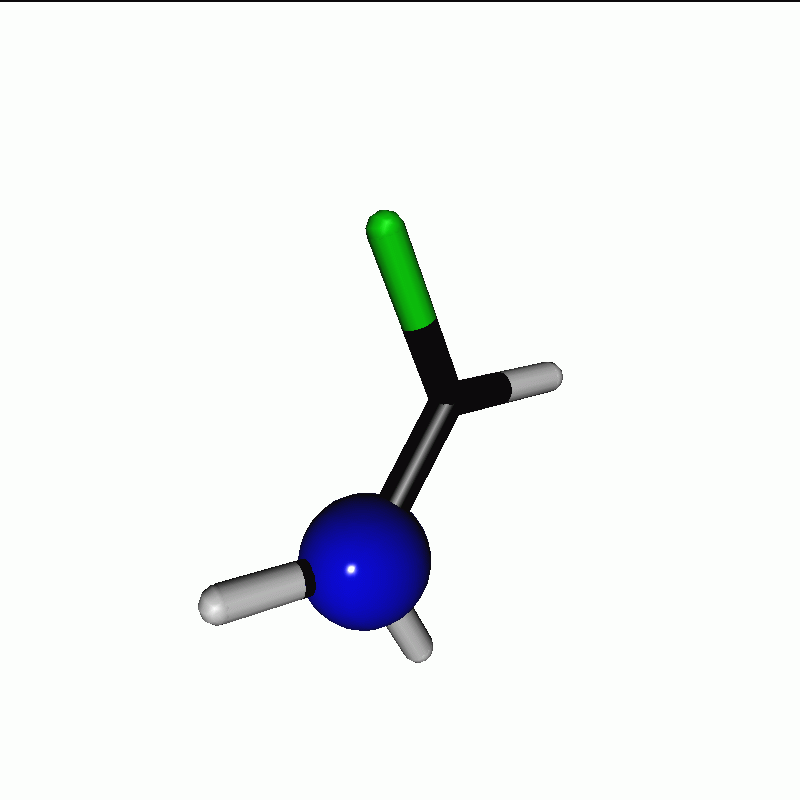
\includegraphics[scale=0.10]{NTO/CH2CHF/1h.png}
     \end{minipage}
     & 0.78
     &  \begin{minipage}{0.2\textwidth}
         \centering
         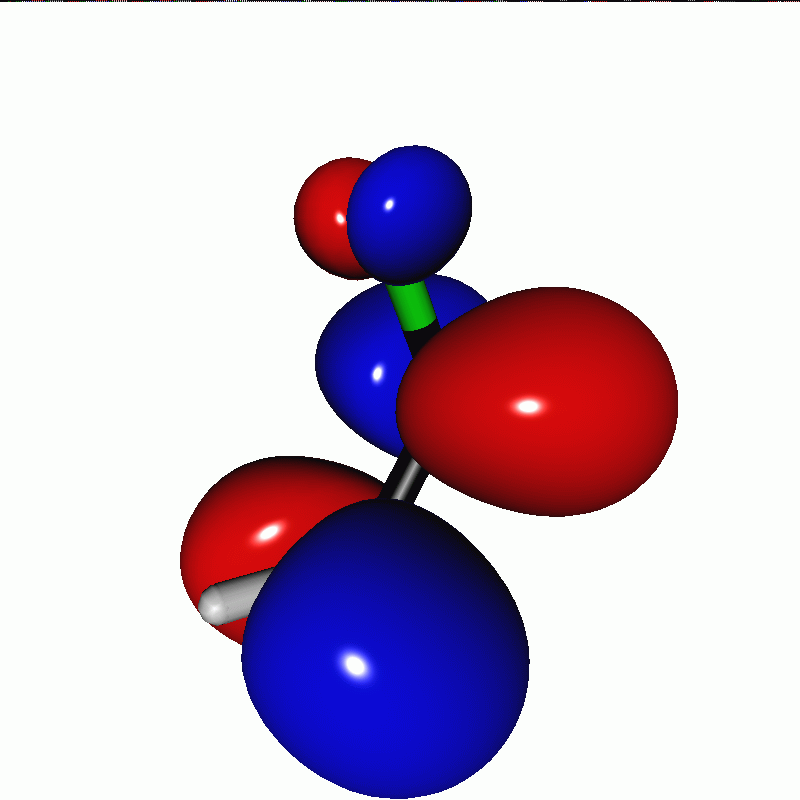
\includegraphics[scale=0.10]{NTO/CH2CHF/1p.png}
     \end{minipage}
     & 105.8
     & 32.5
     & 15.6
     & 153.9
     \\
         B &  
     \begin{minipage}{0.2\textwidth}
         \centering
         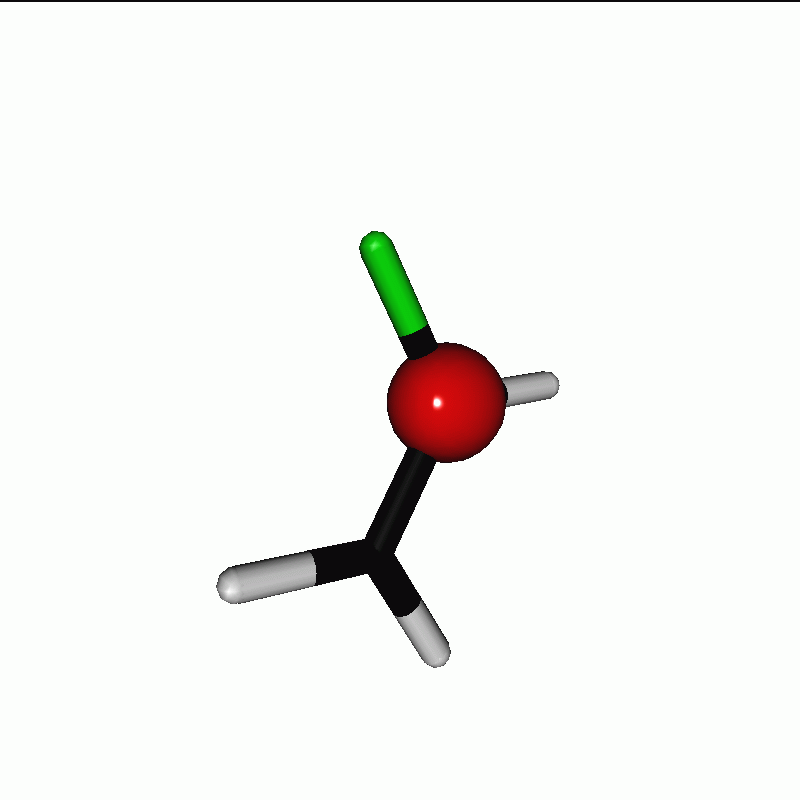
\includegraphics[scale=0.10]{NTO/CH2CHF/2h.png}
     \end{minipage}
     & 0.79
     &  \begin{minipage}{0.2\textwidth}
         \centering
         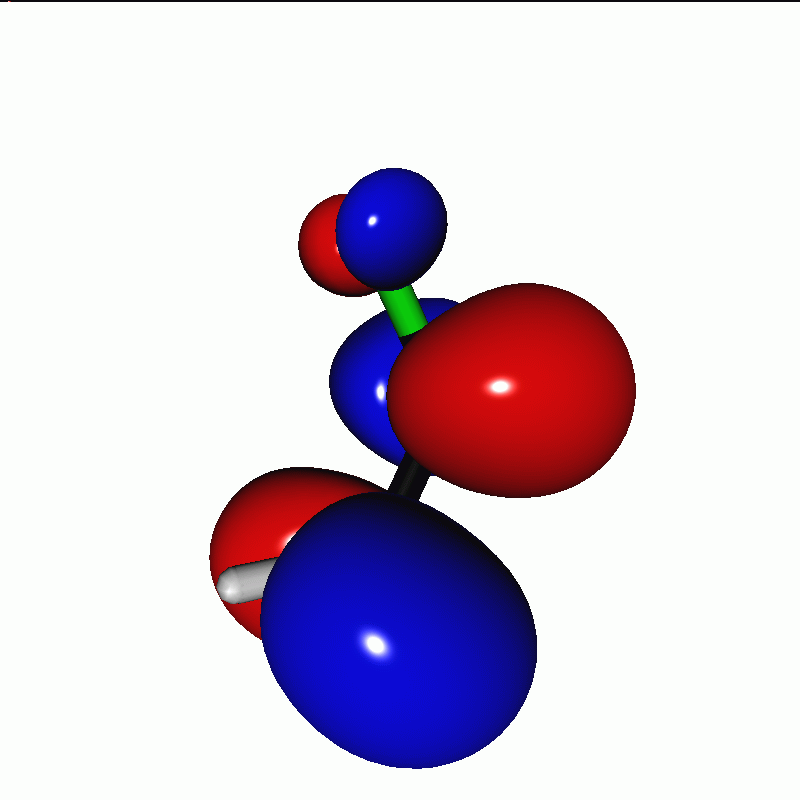
\includegraphics[scale=0.10]{NTO/CH2CHF/2p.png}
     \end{minipage}
     & 108.3
     & 32.1
     & 15.7 
     & 156.1
     \\
             C &  
     \begin{minipage}{0.2\textwidth}
         \centering
         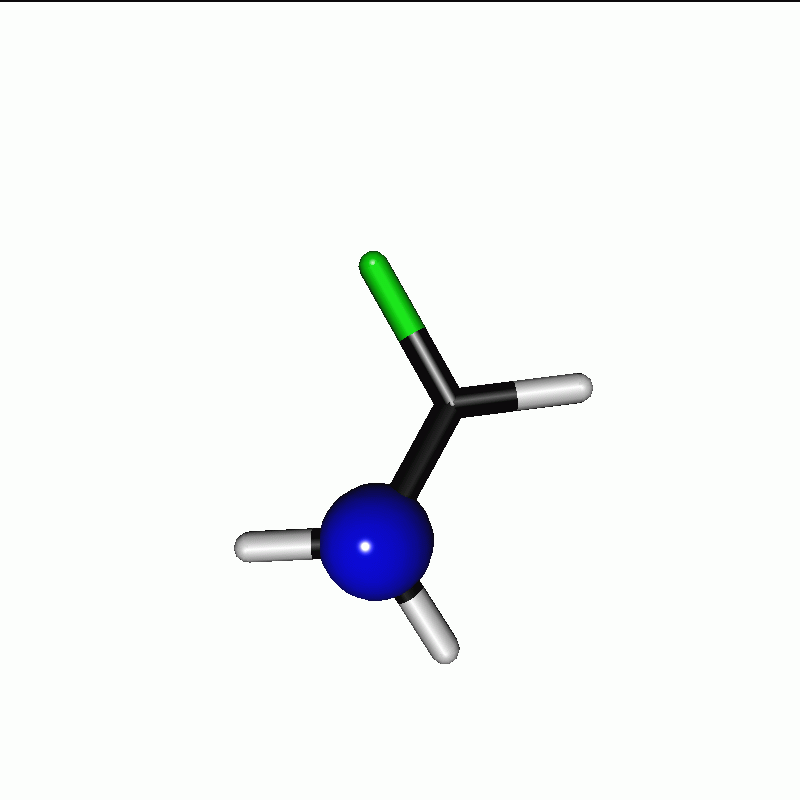
\includegraphics[scale=0.10]{NTO/CH2CHF/4h.png}
     \end{minipage}
     & 0.82
     &  \begin{minipage}{0.2\textwidth}
         \centering
         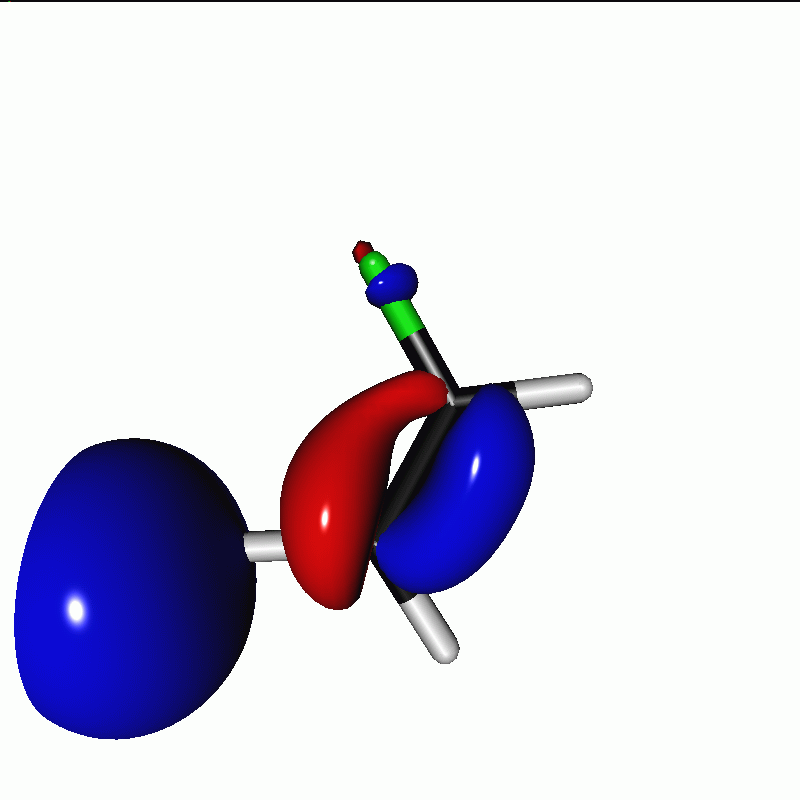
\includegraphics[scale=0.10]{NTO/CH2CHF/4p.png}
     \end{minipage}
     & 112.7
     & 53.4
     & 18.3
     & 184.4
     \\
                  D &  
     \begin{minipage}{0.2\textwidth}
         \centering
         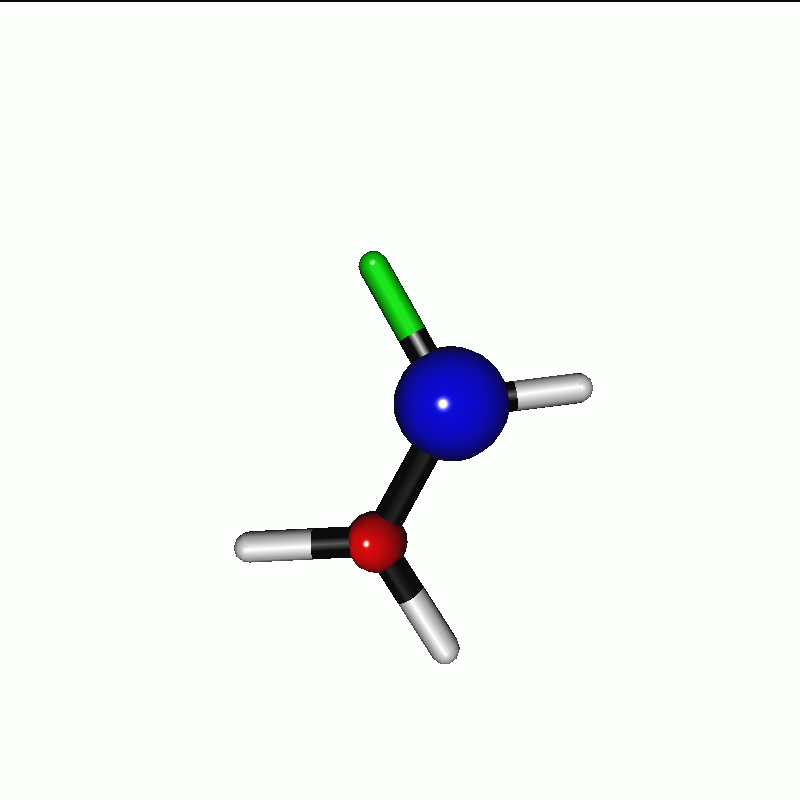
\includegraphics[scale=0.10]{NTO/CH2CHF/8h.png}
         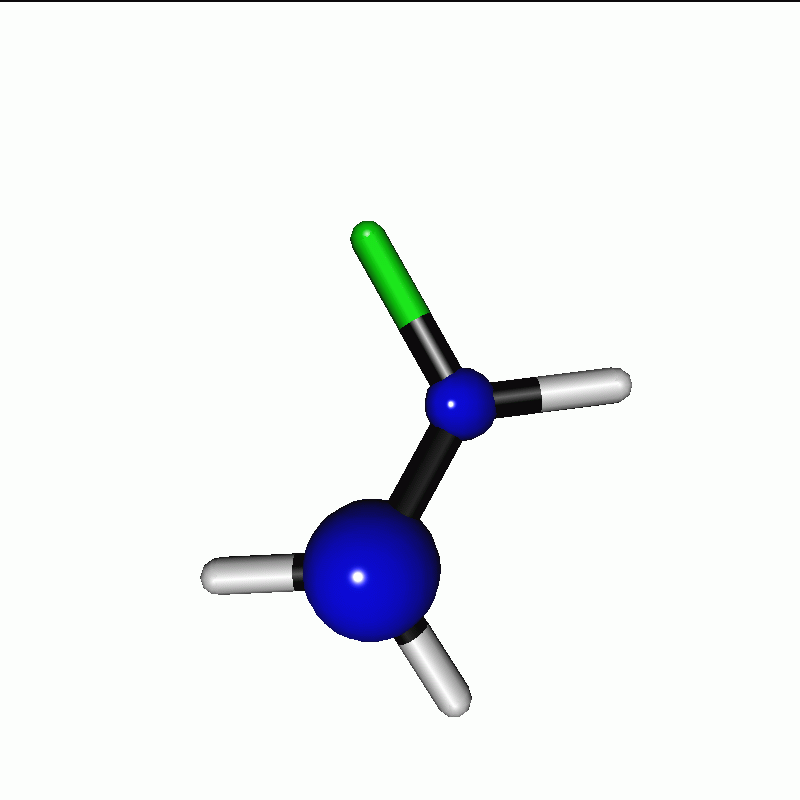
\includegraphics[scale=0.10]{NTO/CH2CHF/8h_019.png}
     \end{minipage}
     &
     \begin{minipage}{0.1\textwidth}
     \centering
      0.62
     \vspace{1cm}
     \\
     \vspace{1cm}
     0.19
     \end{minipage}
     &  \begin{minipage}{0.2\textwidth}
         \centering
         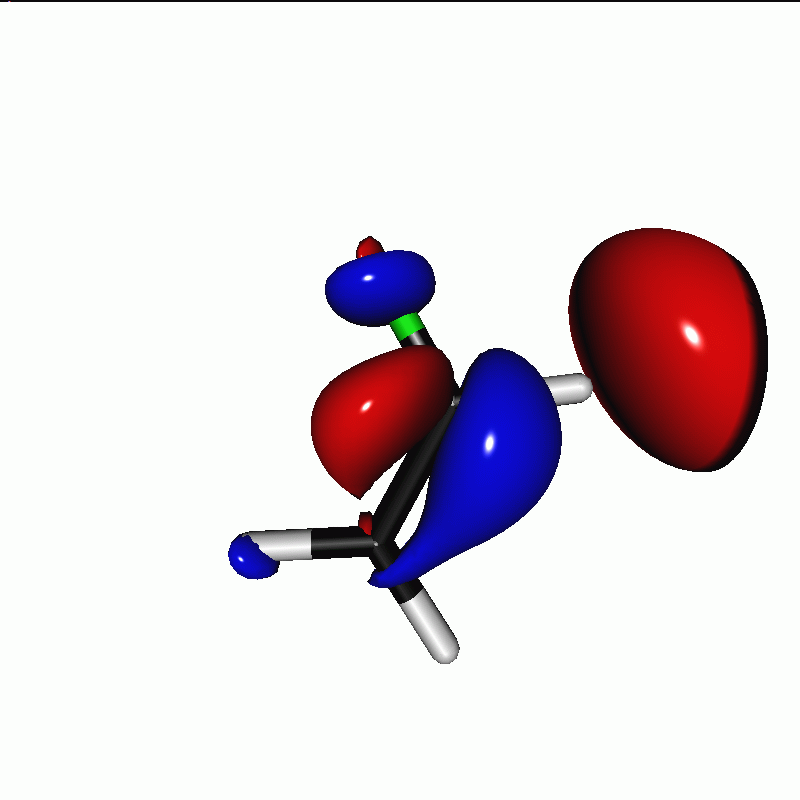
\includegraphics[scale=0.10]{NTO/CH2CHF/8p.png}
         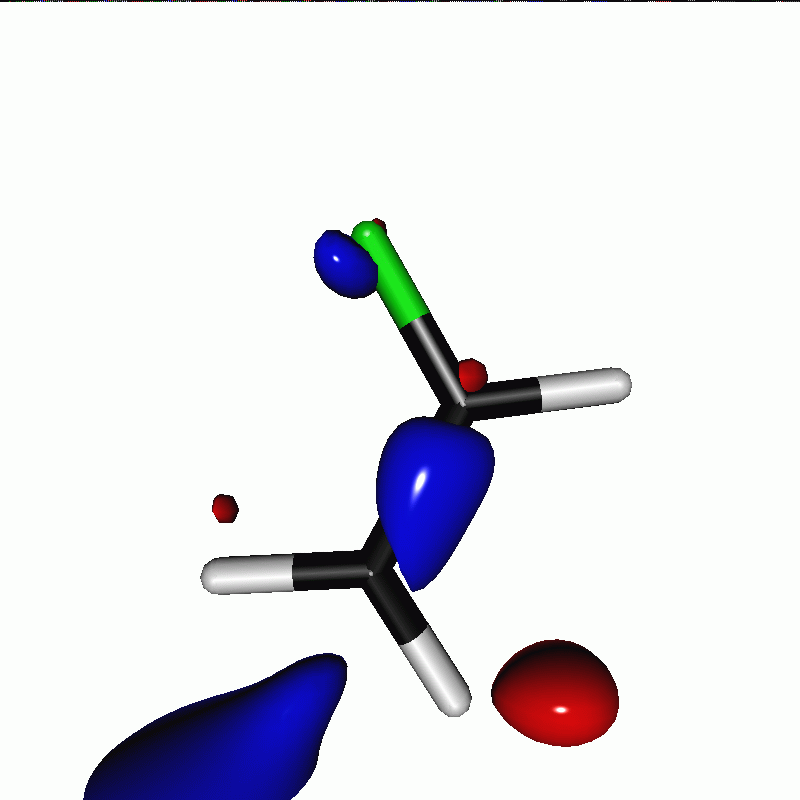
\includegraphics[scale=0.10]{NTO/CH2CHF/8p_019.png}
     \end{minipage}
     & 114.8 & 46.5 & 19.7 & 180.9
     \\
                  E &  
     \begin{minipage}{0.2\textwidth}
         \centering
         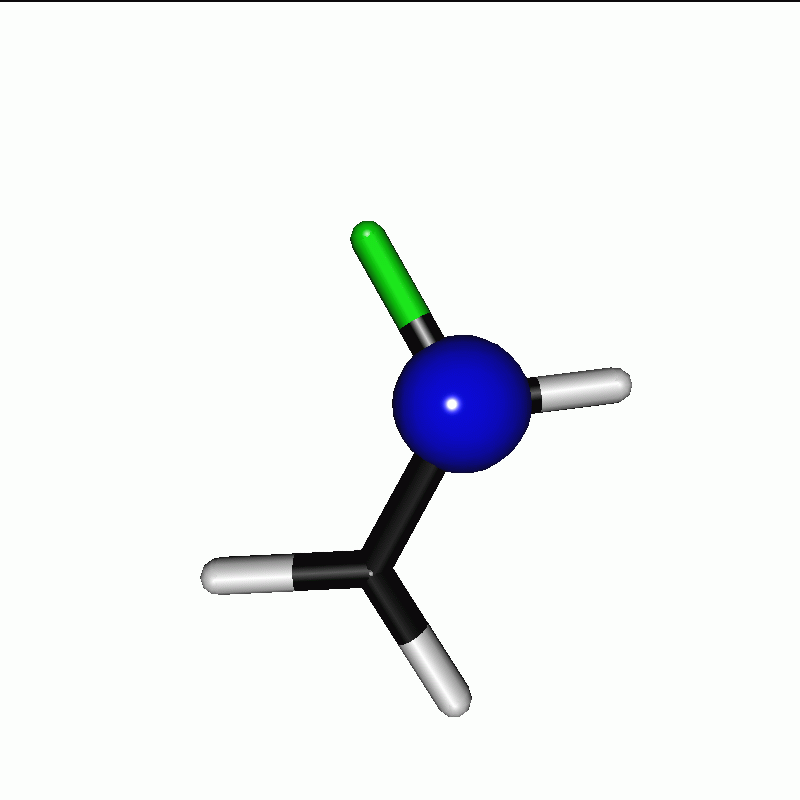
\includegraphics[scale=0.10]{NTO/CH2CHF/11h.png}
     \end{minipage}
     & 0.82
     &  \begin{minipage}{0.2\textwidth}
         \centering
         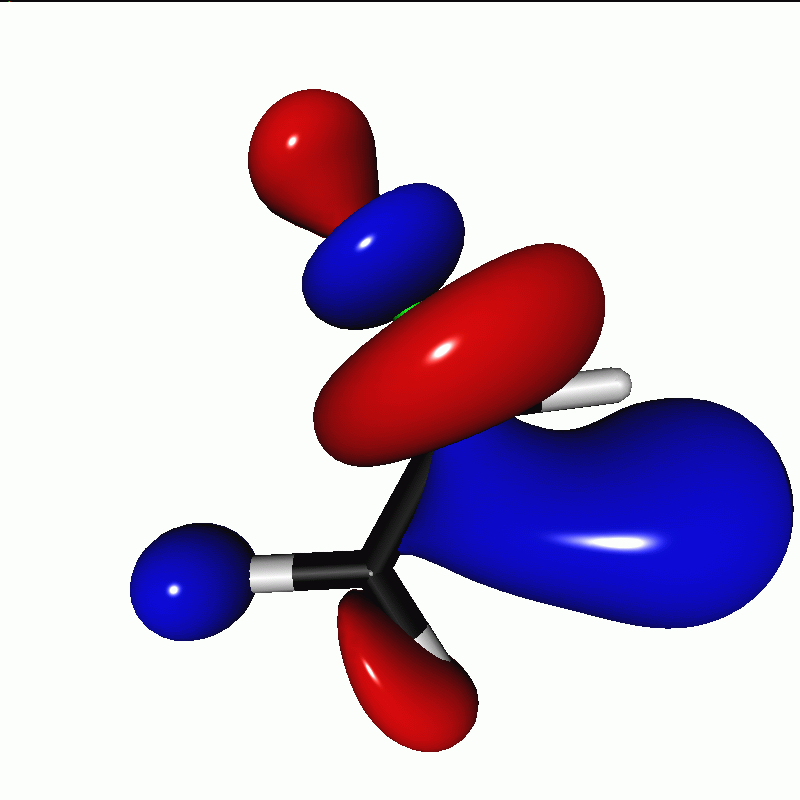
\includegraphics[scale=0.10]{NTO/CH2CHF/11p.png}
     \end{minipage}
     & 111.5 & 41.3 & 17.0 & 186.4
     \\
     \hline
 \end{tabular}
 \end{table}
%
% %Shifted respect to first experimental peak estimated at 688.9 eV
\begin{figure}[H]
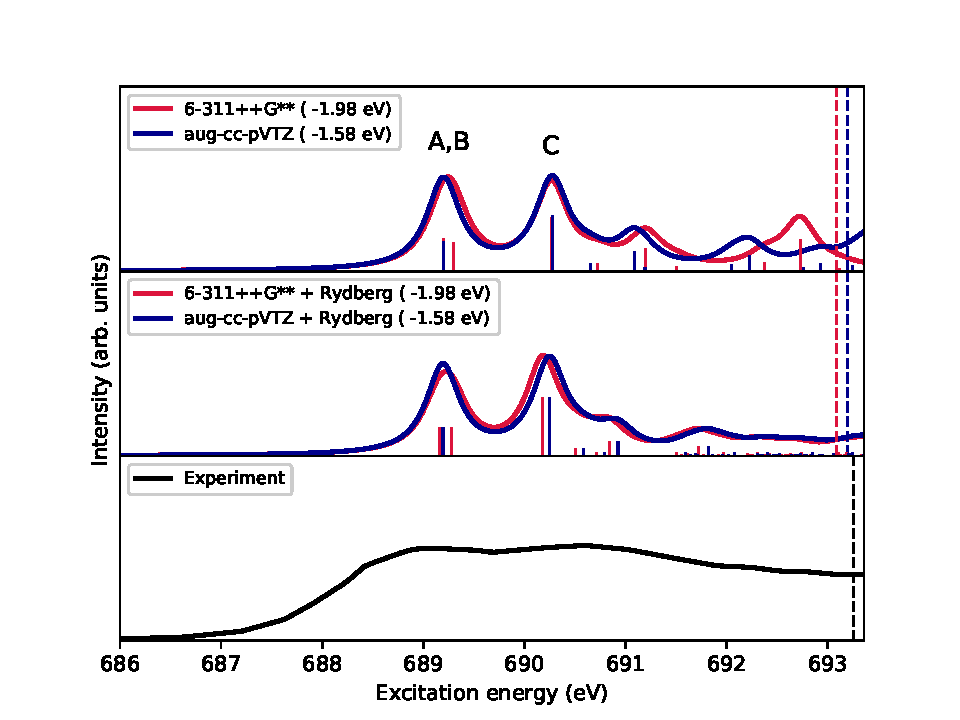
\includegraphics[width=0.9\textwidth]{Spectra/CH2CHF_F.pdf}  
\caption{Vinylfluoride. fc-CVS-EOMEE-CCSD X-ray absorption spectra at the fluorine edge, obtained by convolution of the computed energies and oscillator strengths with a Lorentzian function (FWHM = 0.4 eV). The experimental spectrum was digitized from Ref.~\citenum{NEXAFS_C2H4_CH2CHF_Exp}. 
The dashed vertical lines correspond to the IEs.  
The energy shifts 
required to align the NEXAFS profiles in each basis set with the
experimental one are indicated in parenthesis. The computed IEs have been shifted by the same amount as used to align the NEXAFS profiles. 
The shift was computed based on the experimentally 
derived maximum at 689.2 eV.
\label{fgr:vinylfluoride:F}}
\end{figure}
%
%
\begin{table}[H]
 \centering
 \caption{Vinylfluoride. fc-CVS-EOM-CCSD/6-311++G** 
 NTOs of 3 selected core-excited states at the F edge. 
 NTO isosurface is 0.05\label{vinylfluoride-ntos-Fedge}
 \label{NTOs:fluorine}}
 \vspace{3em}
 \begin{tabular}{ c | c c c }
     \hline
             & \multicolumn{3}{c}{} \\
     State &  Hole & $\sigma_K^2$ & Particle \\
     \hline
     A &  
     \begin{minipage}{0.2\textwidth}
         \centering
         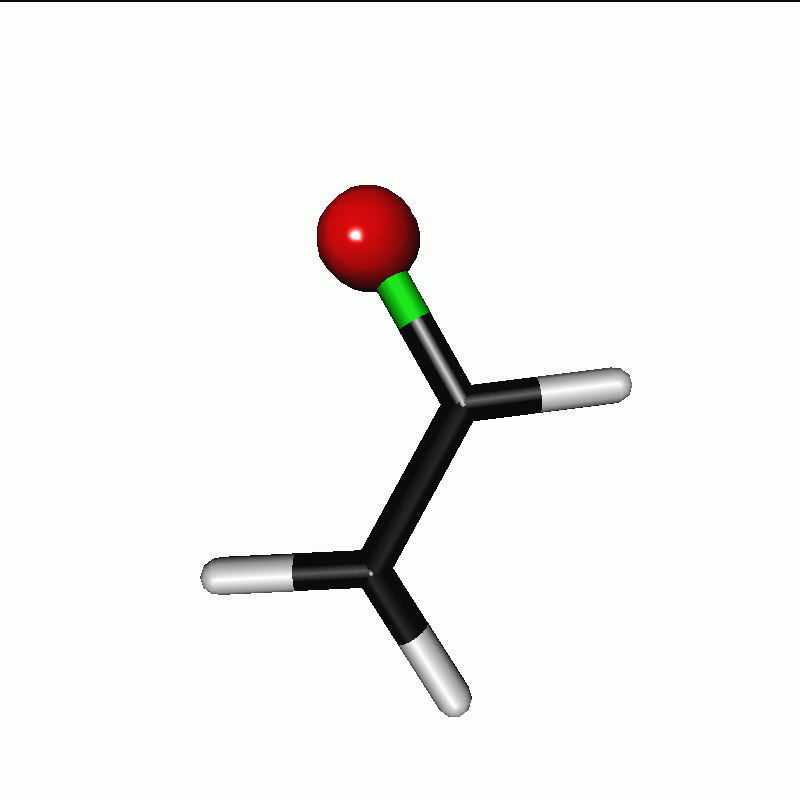
\includegraphics[scale=0.10]{NTO/CH2CHF/CH2CHF_F_1h.png}
     \end{minipage}
     & 0.84
     &  \begin{minipage}{0.2\textwidth}
         \centering
         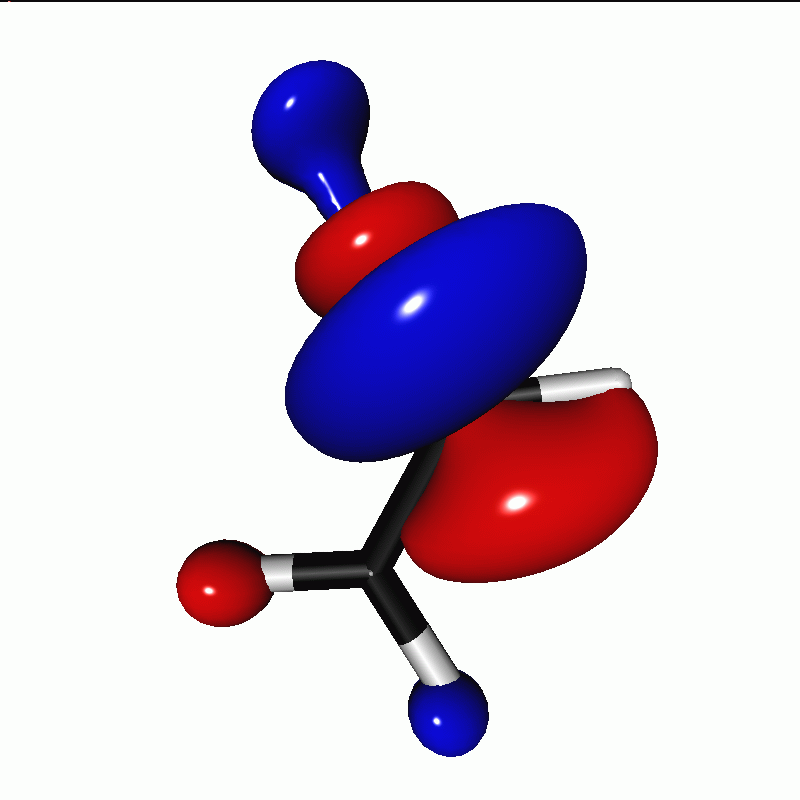
\includegraphics[scale=0.10]{NTO/CH2CHF/CH2CHF_F_1p.png}
     \end{minipage}
     \\
         B &  
     \begin{minipage}{0.2\textwidth}
         \centering
         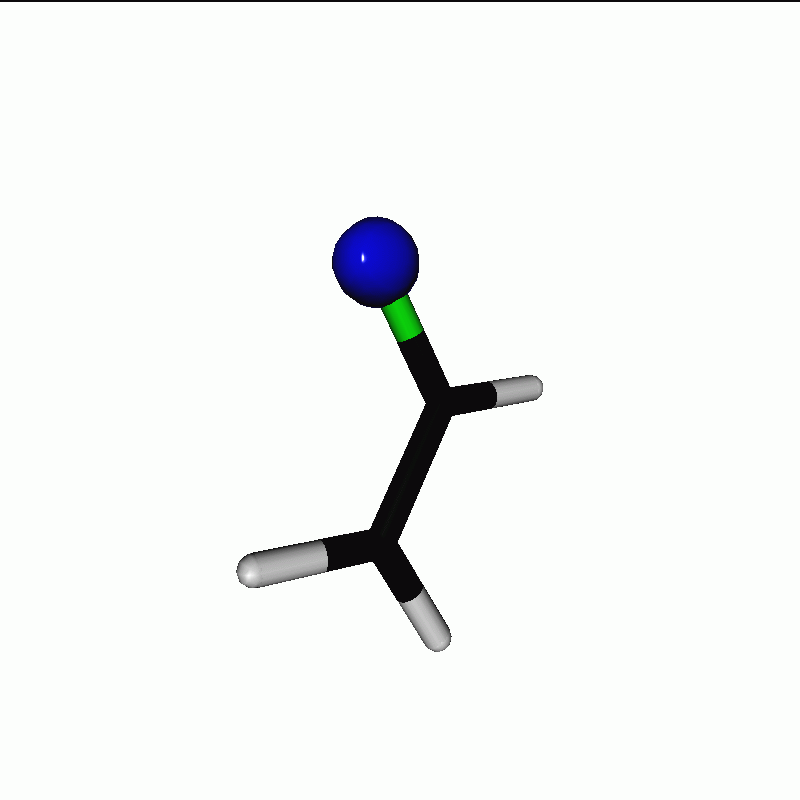
\includegraphics[scale=0.10]{NTO/CH2CHF/CH2CHF_F_2h.png}
     \end{minipage}
     & 0.79
     &  \begin{minipage}{0.2\textwidth}
         \centering
         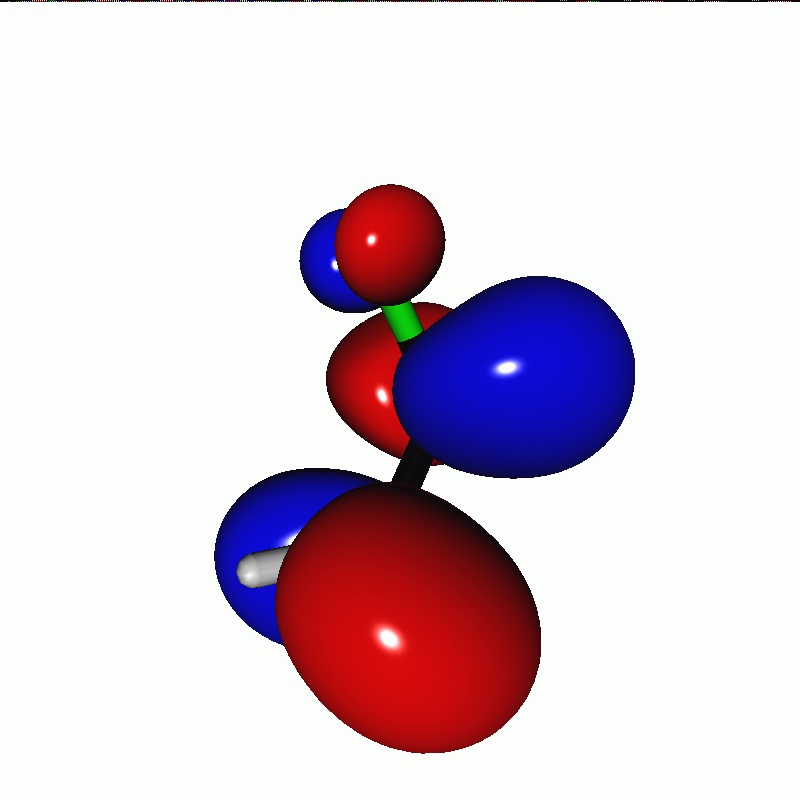
\includegraphics[scale=0.10]{NTO/CH2CHF/CH2CHF_F_2p.png}
     \end{minipage}
     \\
             C &  
     \begin{minipage}{0.2\textwidth}
         \centering
         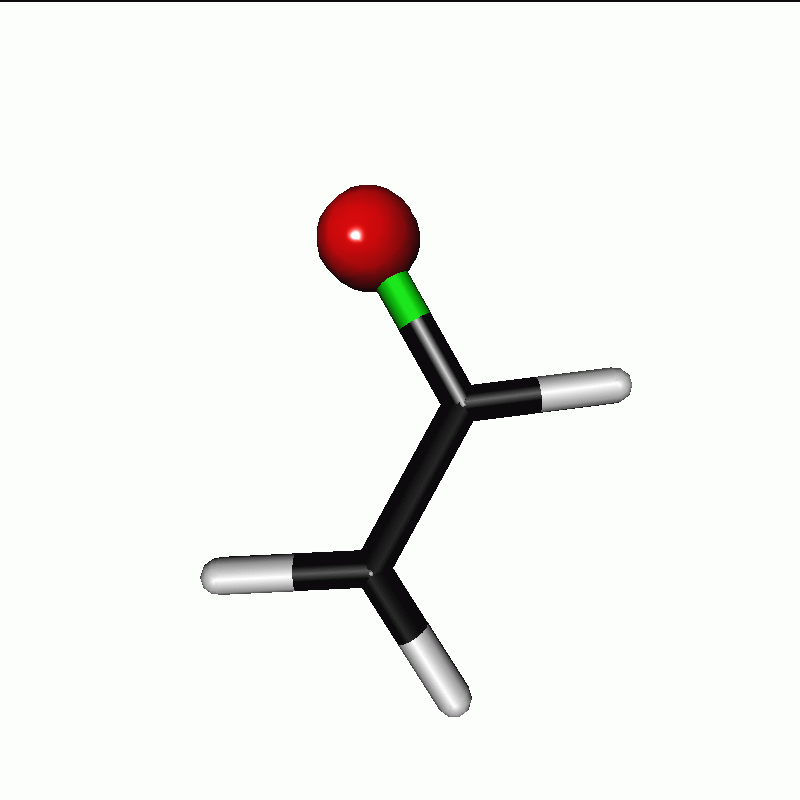
\includegraphics[scale=0.10]{NTO/CH2CHF/CH2CHF_F_3h.png}
     \end{minipage}
     & 0.83·
     &  \begin{minipage}{0.2\textwidth}
         \centering
         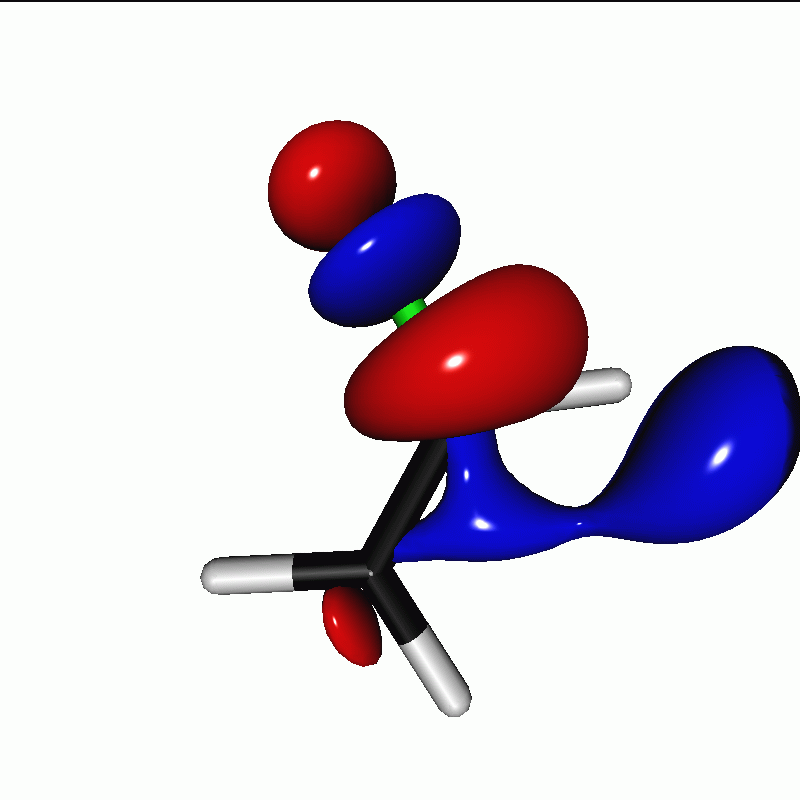
\includegraphics[scale=0.10]{NTO/CH2CHF/CH2CHF_F_3p.png}
     \end{minipage}
     \\
     \hline
 \end{tabular}
 \end{table}
%

\clearpage
%%%%%%%%%%%%%%%%%% OZONE %%%%%%%%%%%%%%%%%%%%%%%%%%%%%
Fig.~\ref{fgr:Ozone} shows the fc-CVS-EOM-CCSD NEXAFS spectra of \ce{O3}, based on the spectral data in Table~\ref{SI-Tab:Ozone}. This molecule displays the largest rigid shifts compared to the experimental spectrum~\cite{ozone_nexafs_xps}, $-2.35$ eV in the Pople set, and $-1.96$ eV with Dunning's set.
%{\color{red}{Not too surprising as \ce{O3} notoriously requires triples for a proper description of its resonance structure?}}
Apart from this, our calculations confirm the assignment in Ref.~\citenum{ozone_nexafs_xps}: the first spectral feature is due to the terminal oxygens' 1$s\to$ $\pi^\star$, whereas the second (broad) band is due to
both the central oxygens 1$s\to$ $\pi^\star$ and the terminal oxygens' 1$s \to \sigma^\star$ excitations, see also the NTOs in Table~\ref{fgr:Ozone-ntos}.
The shoulder at 530.7 eV in the experimental spectrum is known to be due to the O1$s\to \sigma^\star$ transition of a small amount of \ce{O2} present in the sample~\cite{ozone_nexafs_xps}.

%Shifted respect to first experimental peak estimated at 529.2 eV
\begin{figure}
  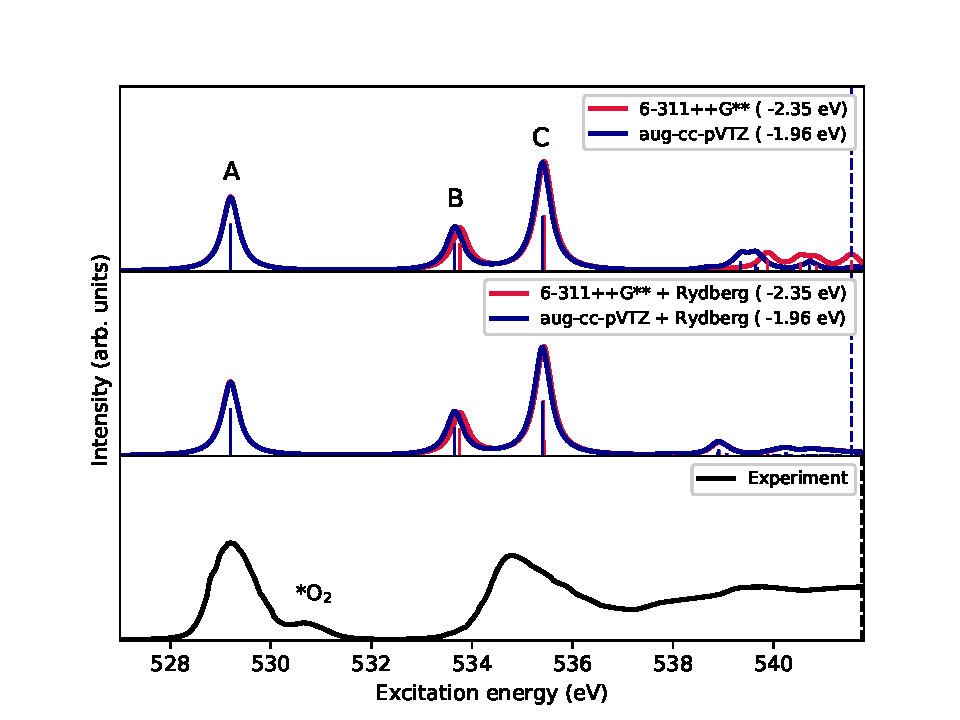
\includegraphics[width=1\textwidth]{Spectra/O3.pdf}  
  \caption{Ozone. fc-CVS-EOMEE-CCSD X-ray absorption spectra obtained from convolution with a Lorentzian function (FWHM = 0.4 eV) of the computed excitation energies and oscillator strengths. The experimental spectrum was digitized from Ref.~\citenum{ozone_nexafs_xps}. The dashed vertical lines correspond to the ionization energy of the terminal O atom. The central oxygen's IE was omitted in figures as it lies above 545 eV.}
  \label{fgr:Ozone}
\end{figure}



\begin{table}[H]
\centering
\caption{Ozone. fc-CVS-EOM-CCSD/6-311++G**   NTOs of the first 3 core-excited states. NTO isosurface is 0.05\label{fgr:Ozone-ntos}}
\vspace{3em}
\begin{tabular}{ c | c c c }
    \hline
            & \multicolumn{3}{c}{} \\
    State &  Hole & $\sigma_K^2$ & Particle \\
    \hline
    A &  
    \begin{minipage}{0.2\textwidth}
        \centering
        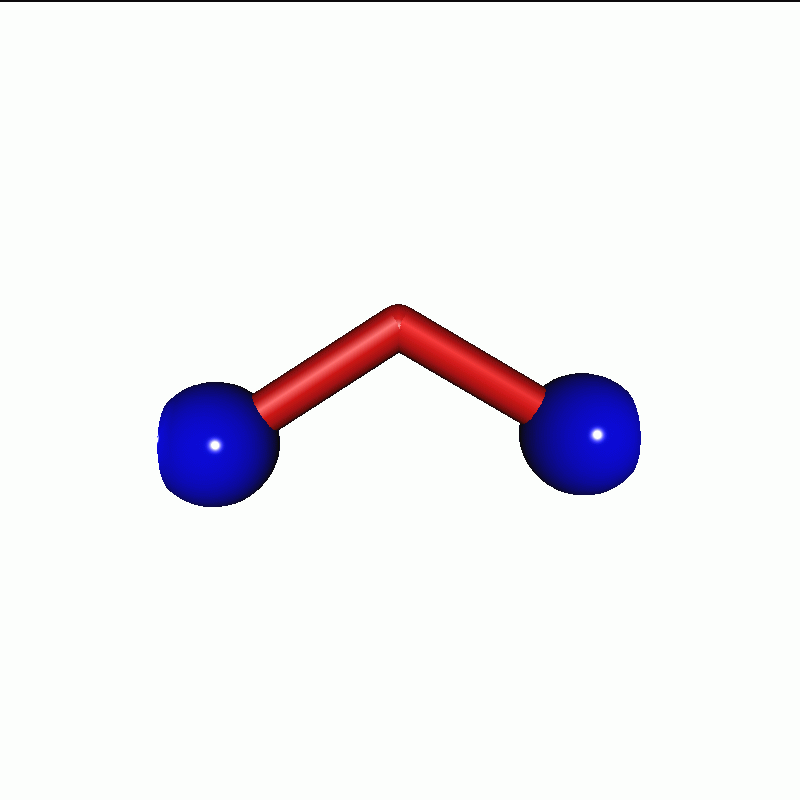
\includegraphics[scale=0.10]{NTO/O3/1h.png}
    \end{minipage}
    &
    0.70
    &  \begin{minipage}{0.2\textwidth}
        \centering
        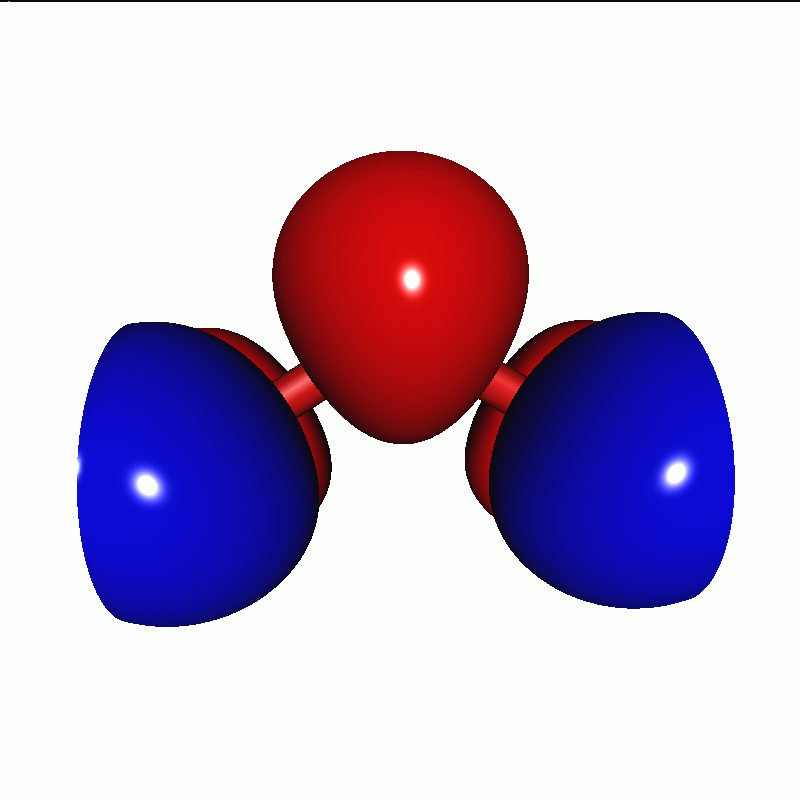
\includegraphics[scale=0.10]{NTO/O3/1p.png}
    \end{minipage}
    \\
        B &  
    \begin{minipage}{0.2\textwidth}
        \centering
        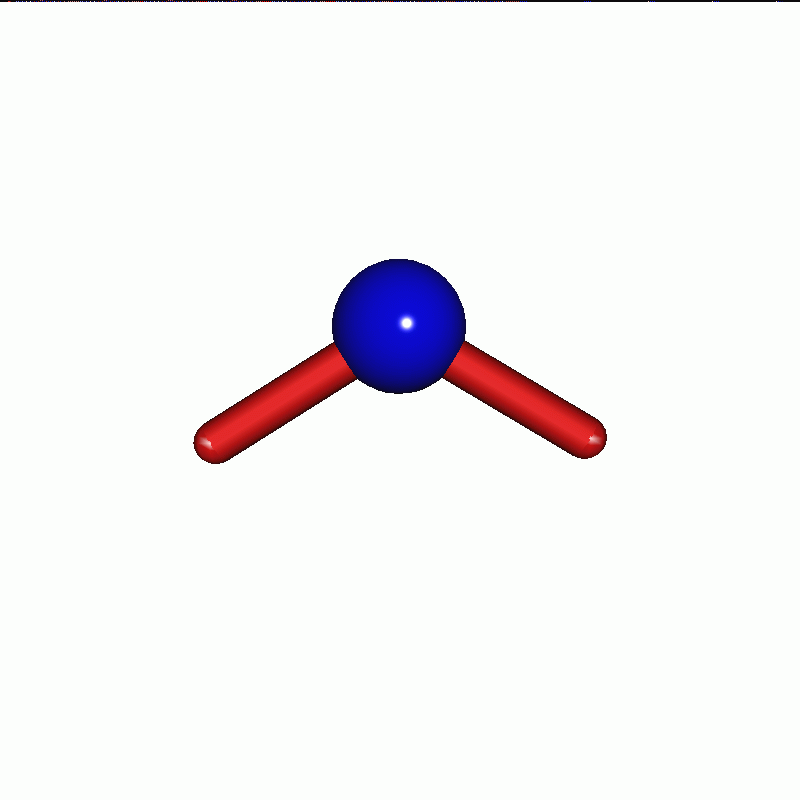
\includegraphics[scale=0.10]{NTO/O3/2h.png}
    \end{minipage}
    &
    0.72 
    &  \begin{minipage}{0.2\textwidth}
        \centering
        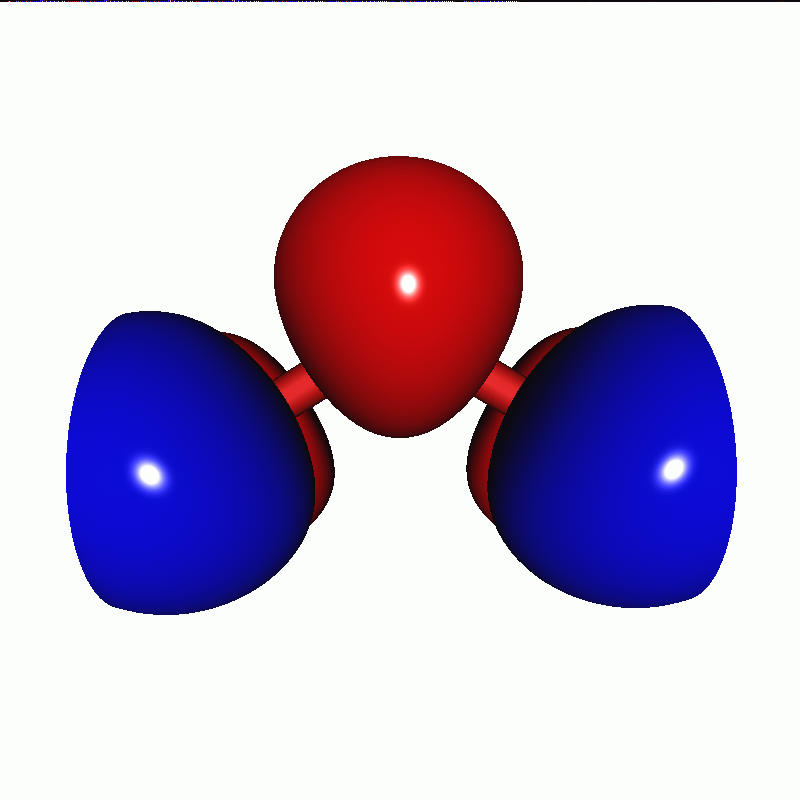
\includegraphics[scale=0.10]{NTO/O3/2p.png}
    \end{minipage}
    \\
            C	 &  
    \begin{minipage}{0.2\textwidth}
        \centering
        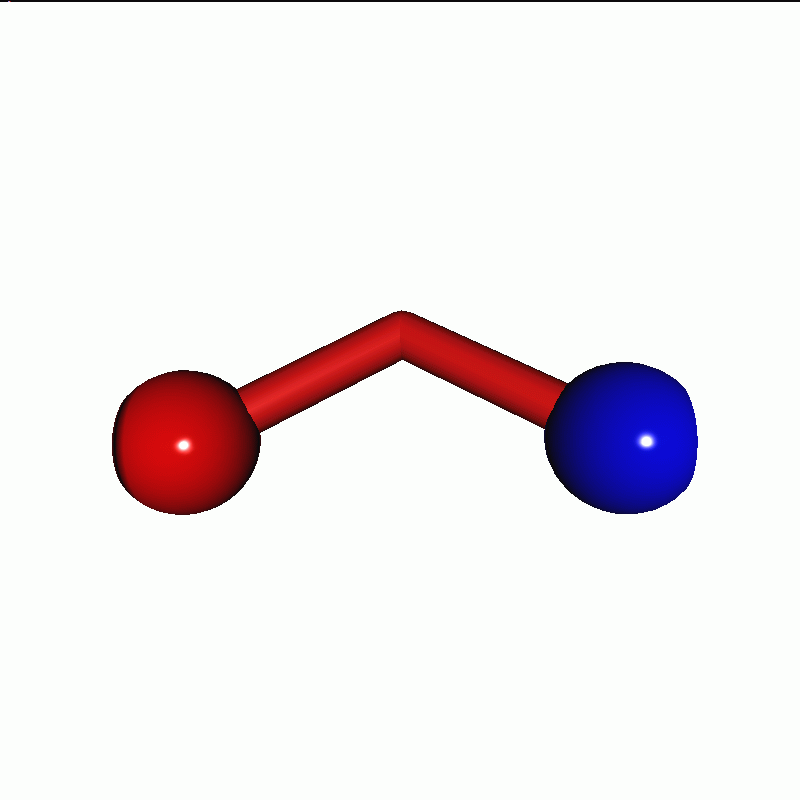
\includegraphics[scale=0.10]{NTO/O3/3h_063.png}
        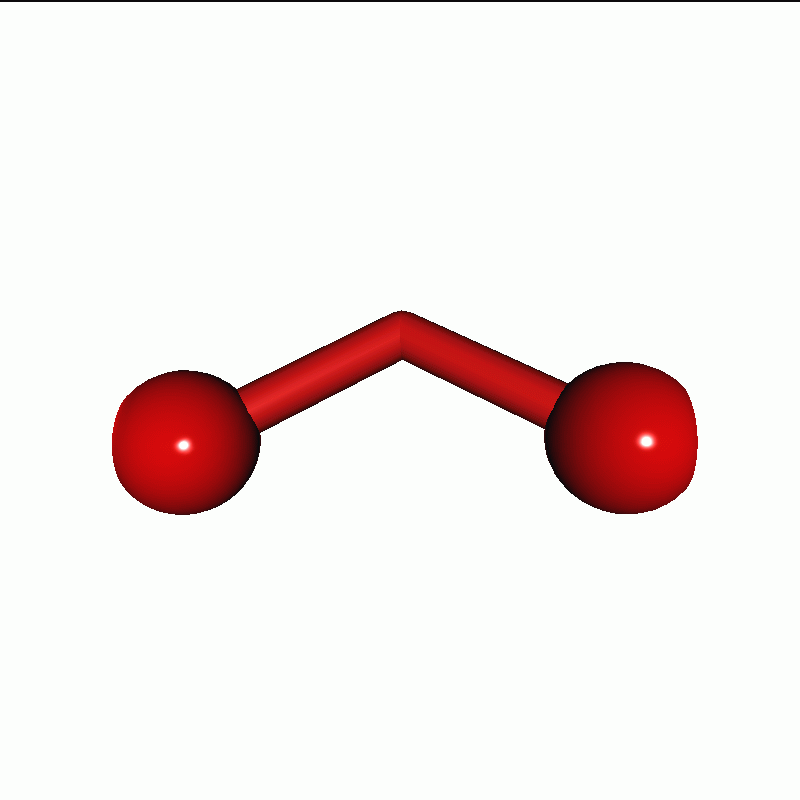
\includegraphics[scale=0.10]{NTO/O3/3h_019.png}
  \end{minipage}
    &
    \begin{minipage}{0.1\textwidth}
        \centering
    0.63 
    \vspace{1cm}
    \\
    \vspace{1cm}
    0.19
    \end{minipage}
    &  \begin{minipage}{0.2\textwidth}
        \centering
        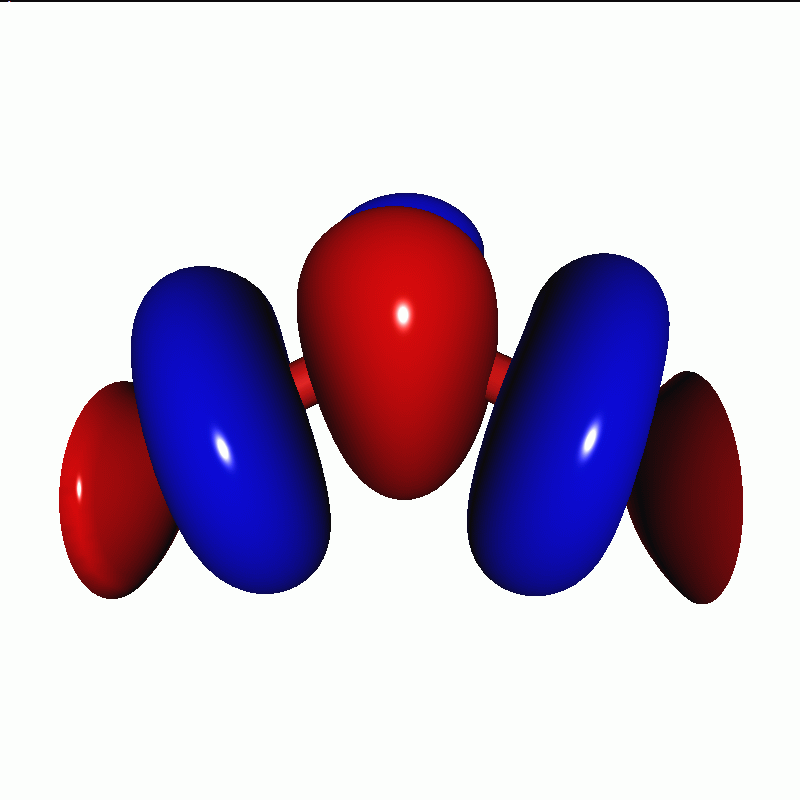
\includegraphics[scale=0.10]{NTO/O3/3p_063.png}
        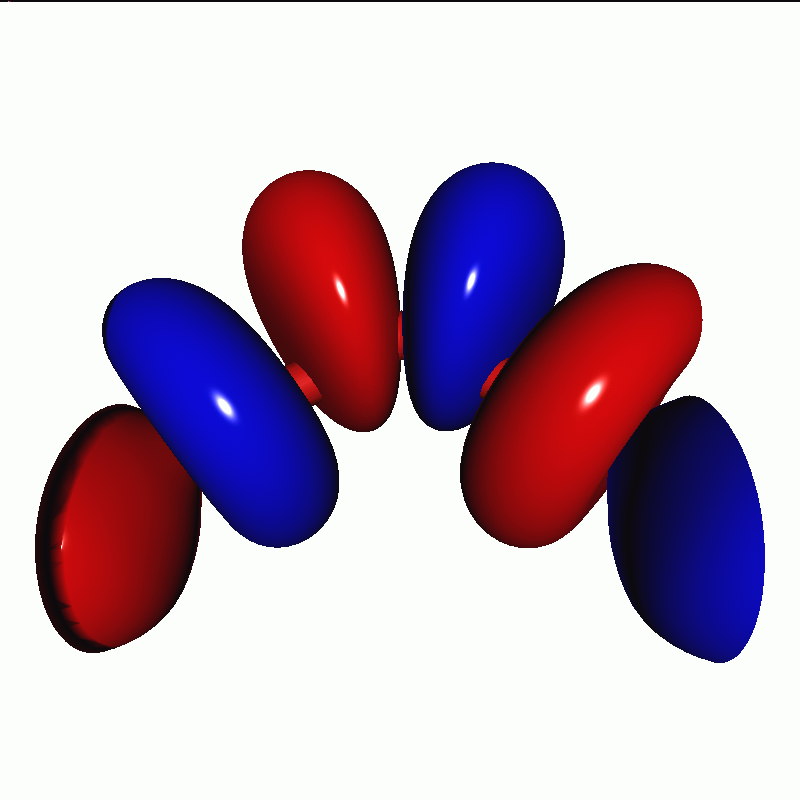
\includegraphics[scale=0.10]{NTO/O3/3p_019.png}  
    \end{minipage}

    \\
    \hline
\end{tabular}
\end{table}

%%%%%%%%%%%%%% Adenine %%%%%%%%%%%%%%
The final system considered here is adenine, whose NEXAFS and XPS spectra were experimentally recorded in gas-phase by \citeauthor{nexafs_thymine_adenine}~\cite{nexafs_thymine_adenine} 
Adenine has also been recently used to test the performance of the variational, time-independent, Orthogonality Constrained
DFT method of Evangelista and co-workers~\cite{derricotte2015simulation}.
We considered both carbon and nitrogen edges. Due to the relative large size of the system, calculations were only performed in the 6-311++G** basis set. 
The C and N K-edge spectra are shown in the upper and lower panels of Figure~\ref{fgr:Adenine}, respectively. The raw data are given in Table~\ref{SI-Tab:Adenine}.
The C K-edge spectra were shifted by $-1.10$(non-planar)/$-1.14$(planar) eV,
and the N K-edge one by $-1.43$(non-planar)/$-1.45$(planar) eV, 
and one can expect an even smaller shift had the larger aug-cc-pVTZ basis set been used.
The experimental features are, once again, quite well reproduced. Remarkably, the C-edge spectrum obtained from the planar geometry is more similar to the experimental spectrum, primarily due to the larger splitting between the 4th and 5th excitations in the non-planar structure. The spectral assignment for both structures is, nonetheless, identical. This is best appreciated looking at the NTOs for the  first 5 excitations shown in Table~\ref{adenine-ntos-Cedge}.
We also note that in this case, as in other examples, NTOs reveal that the electronic transitions have rather simple character and can be described by a single NTO pair. In contrast, the EOM wavefunctions often show mutiple amplitudes with comparable weights, giving a misleading impression of the character of the transition. 

%Shifted respect to first experimental peak estimated at 286.4 eV for the C-edge and 399.4 eV for the N-edge
\begin{figure}[H]
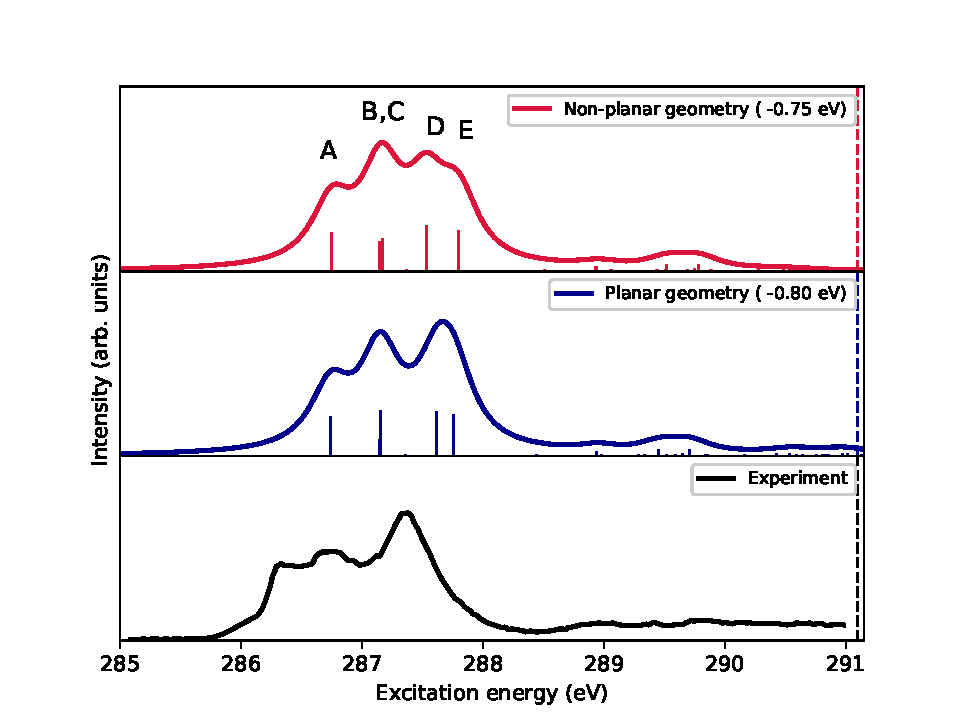
\includegraphics[width=0.75\textwidth]{Spectra/Adenine_C.pdf}
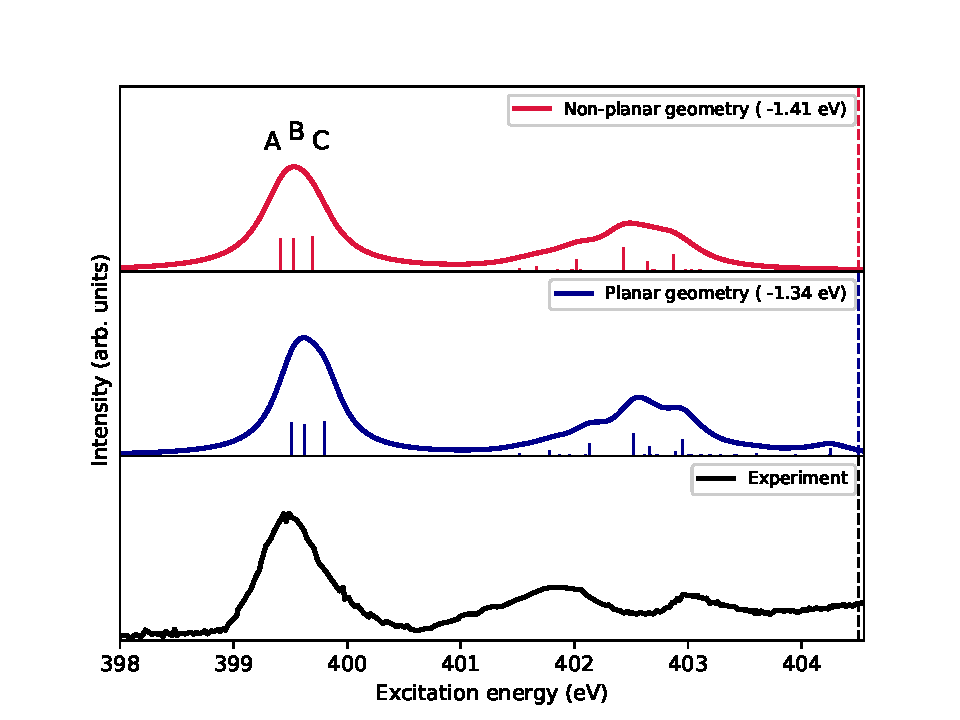
\includegraphics[width=0.75\textwidth]{Spectra/Adenine_N.pdf}
\caption{Adenine. C-edge (upper panels) and N-edge (lower panels) 
fc-CVS-EOMEE-CCSD/6-31++G** X-ray absorption spectra for two different molecular structures, obtained by convolution of the computed energies and oscillator strengths with a Lorentzian function (FWHM = 0.4 eV). The rigid shifts applied are indicated in parenthesis in the legends. They were determined with respect to the first experimental peak position in each spectrum, estimated to be at 286.4 eV for C and 399.4 eV for N.
The vertical dashed line correspond to the first IE. 
The computed IEs have been shifted by the same amount as used to align the NEXAFS profiles.
The experimental spectra were digitized from Ref.~\citenum{nexafs_thymine_adenine}.
\label{fgr:Adenine}}
\end{figure}


\begin{table}[H]
\centering
\caption{Adenine. fc-CVS-EOM-CCSD/6-311++G** NTOs of the first 5 core-excited states at the C K-edge at the non-planar RI-MP2/cc-pVTZ geometry (left) and planar B3LYP/cc-pVTZ geometry (right). NTO isosurface is 0.05.\label{adenine-ntos-Cedge}}
\vspace{3em}
\small
\begin{tabular}{ l| c c c | c c c }
\hline
& \multicolumn{3}{c}{Non-planar} & \multicolumn{3}{|c}{Planar} \\
    State &  Hole &$\sigma_K^2$& Particle & Hole &$\sigma_K^2$& Particle \\
    \hline
    A &  
    \begin{minipage}{0.2\textwidth}
        \centering
        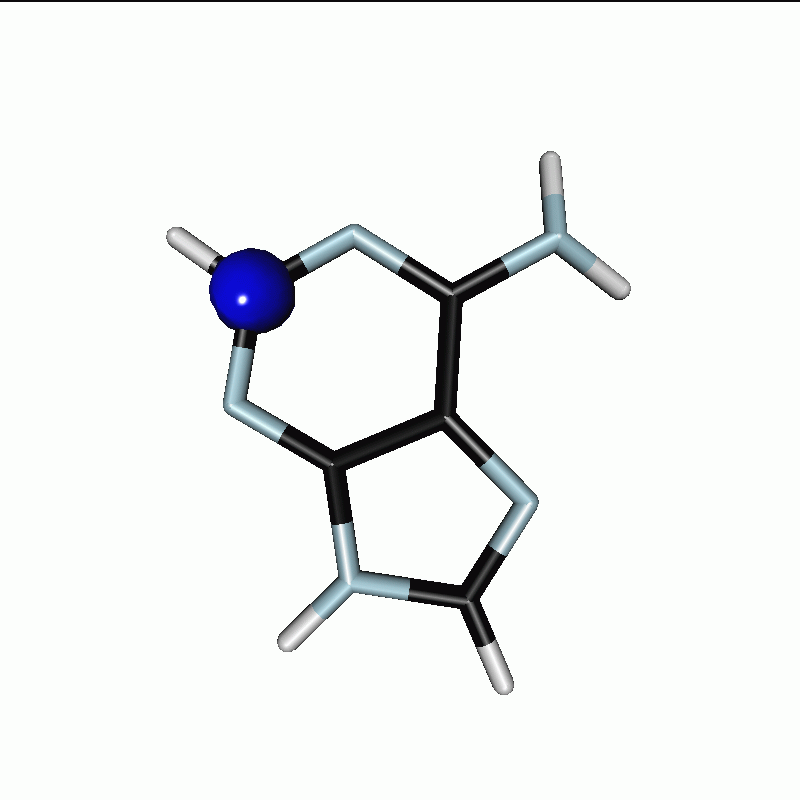
\includegraphics[scale=0.10]{NTO/Adenine_C/1h_C1.png}
    \end{minipage}
    & 0.81
    &  \begin{minipage}{0.2\textwidth}
        \centering
        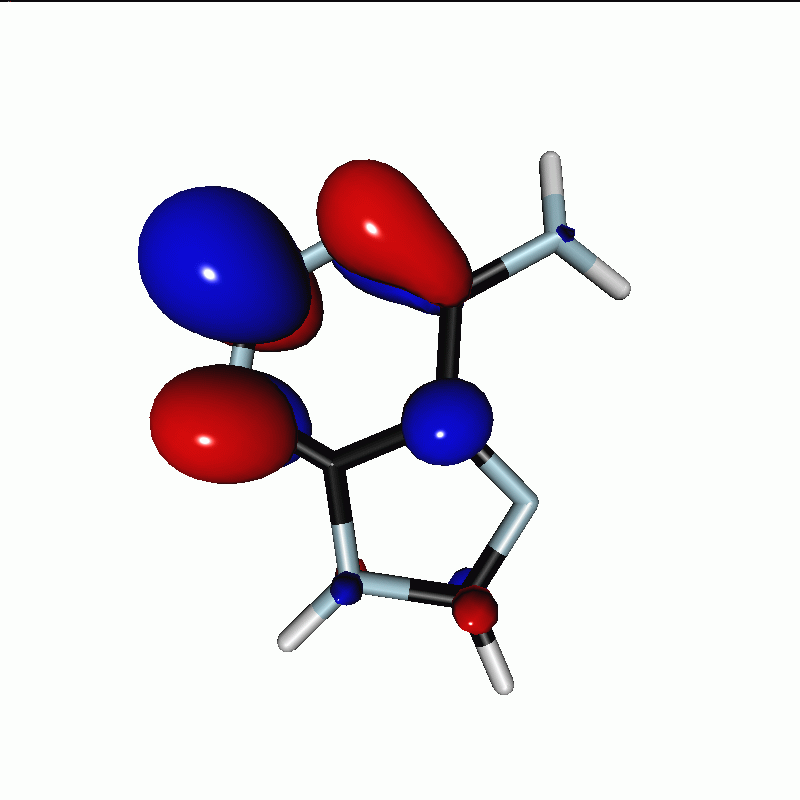
\includegraphics[scale=0.10]{NTO/Adenine_C/1p_C1.png}
    \end{minipage}
    & 
    \begin{minipage}{0.2\textwidth}
        \centering
        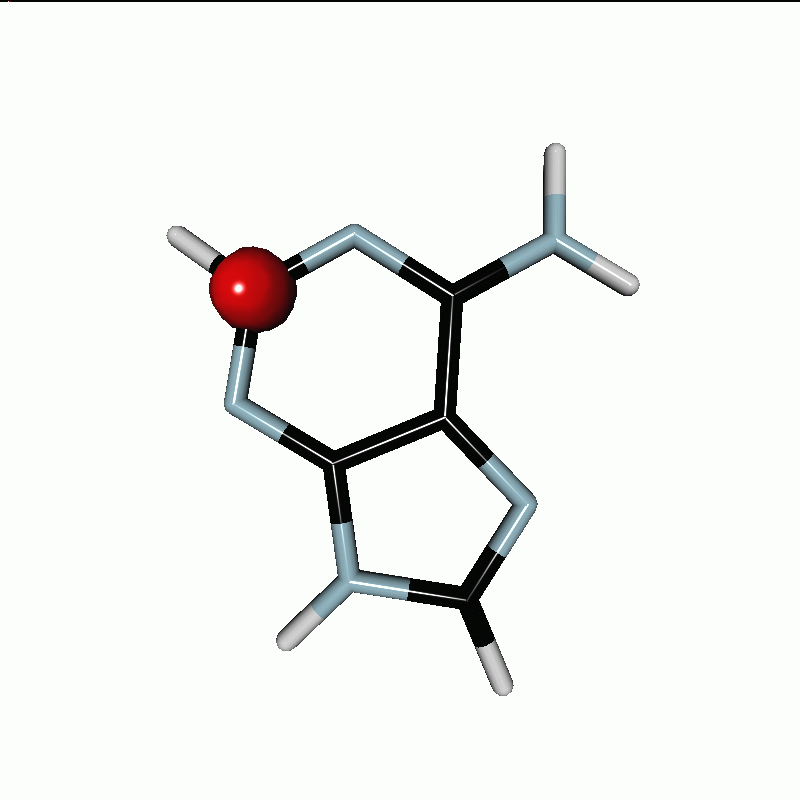
\includegraphics[scale=0.10]{NTO/Adenine_C/1h_Cs.png}
    \end{minipage}
    & 0.81
    & 
    \begin{minipage}{0.2\textwidth}
        \centering
        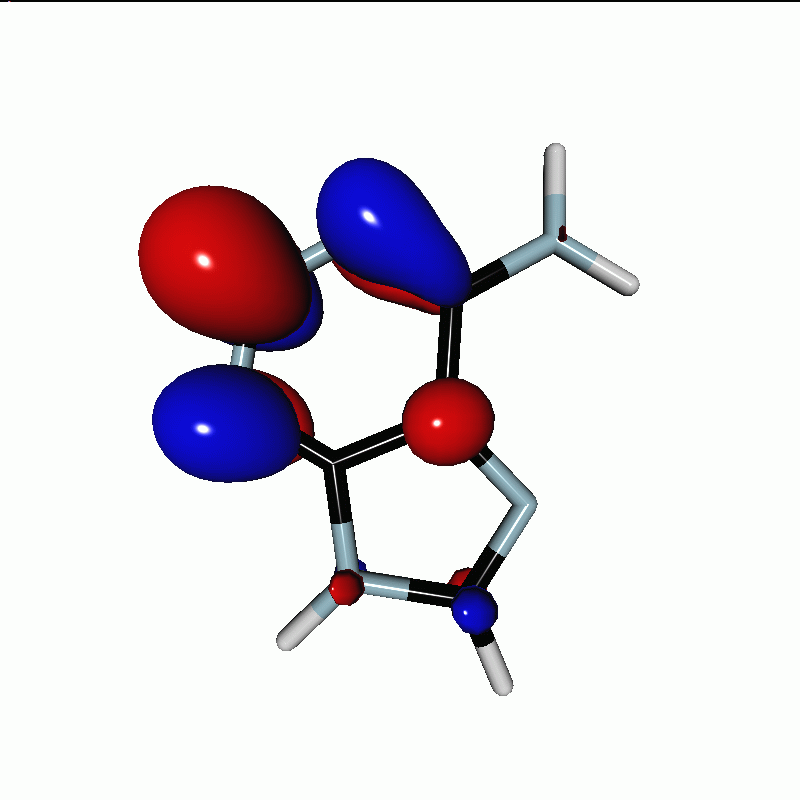
\includegraphics[scale=0.10]{NTO/Adenine_C/1p_Cs.png}
    \end{minipage}
    \\
        B &  
    \begin{minipage}{0.2\textwidth}
        \centering
        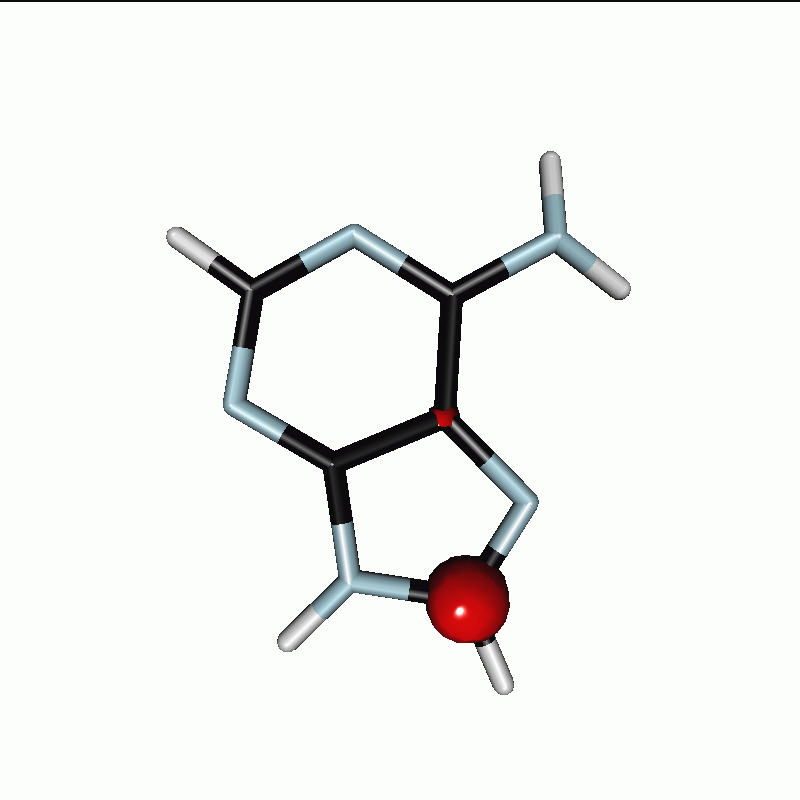
\includegraphics[scale=0.10]{NTO/Adenine_C/2h_C1.png}
    \end{minipage}
    & 0.79
    &  \begin{minipage}{0.2\textwidth}
        \centering
        \includegraphics[scale=0.10]{NTO/Adenine_C/2p_C1.png}
    \end{minipage}
    & 
    \begin{minipage}{0.2\textwidth}
        \centering
        \includegraphics[scale=0.10]{NTO/Adenine_C/2h_Cs.png}
    \end{minipage}
    & 0.71
    & 
    \begin{minipage}{0.2\textwidth}
        \centering
        \includegraphics[scale=0.10]{NTO/Adenine_C/2p_Cs.png}
    \end{minipage}
    \\
            C &  
    \begin{minipage}{0.2\textwidth}
        \centering
        \includegraphics[scale=0.10]{NTO/Adenine_C/3h_C1.png}
    \end{minipage}
    & 0.77
    &  \begin{minipage}{0.2\textwidth}
        \centering
        \includegraphics[scale=0.10]{NTO/Adenine_C/3p_C1.png}
    \end{minipage}
    & 
    \begin{minipage}{0.2\textwidth}
        \centering
        \includegraphics[scale=0.10]{NTO/Adenine_C/3h_Cs.png}
    \end{minipage}
    & 0.71
    & 
    \begin{minipage}{0.2\textwidth}
        \centering
        \includegraphics[scale=0.10]{NTO/Adenine_C/3p_Cs.png}
    \end{minipage}
    \\
            D &  
    \begin{minipage}{0.2\textwidth}
        \centering
        \includegraphics[scale=0.10]{NTO/Adenine_C/5h_C1.png}
    \end{minipage}
    & 0.75
    &  \begin{minipage}{0.2\textwidth}
        \centering
        \includegraphics[scale=0.10]{NTO/Adenine_C/5p_C1.png}
    \end{minipage}
    & 
    \begin{minipage}{0.2\textwidth}
        \centering
        \includegraphics[scale=0.10]{NTO/Adenine_C/5h_Cs.png}
    \end{minipage}
    & 0.82
    & 
    \begin{minipage}{0.2\textwidth}
        \centering
        \includegraphics[scale=0.10]{NTO/Adenine_C/5p_Cs.png}
    \end{minipage}
    \\
            E &  
    \begin{minipage}{0.2\textwidth}
        \centering
        \includegraphics[scale=0.10]{NTO/Adenine_C/6h_C1.png}
    \end{minipage}
    & 0.81
    &  \begin{minipage}{0.2\textwidth}
        \centering
        \includegraphics[scale=0.10]{NTO/Adenine_C/6p_C1.png}
    \end{minipage}
    & 
    \begin{minipage}{0.2\textwidth}
        \centering
        \includegraphics[scale=0.10]{NTO/Adenine_C/6h_Cs.png}
    \end{minipage}
    & 0.81
    & 
    \begin{minipage}{0.2\textwidth}
        \centering
        \includegraphics[scale=0.10]{NTO/Adenine_C/6p_Cs.png}
    \end{minipage}
    \\
    \hline
\end{tabular}
\end{table}

\begin{table}[H]
\centering
\caption{Adenine. fc-CVS-EOM-CCSD/6-311++G** NTOs of the first 3 core-excited states at the N K-edge at the non-planar RI-MP2/cc-pVTZ geometry (left) and planar B3LYP/cc-pVTZ geometry. NTO isosurface is 0.05.\label{adenine-ntos-Nedge}}
\vspace{3em}
\small
\begin{tabular}{ l | c c c | c c c }
    \hline
            & \multicolumn{3}{c}{Non-planar} & \multicolumn{3}{|c}{Planar} \\
    State &  Hole &$\sigma_K^2$& Particle & Hole &$\sigma_K^2$& Particle \\
    \hline
    A &  
    \begin{minipage}{0.2\textwidth}
        \centering
        \includegraphics[scale=0.10]{NTO/Adenine_N/1h_C1.png}
    \end{minipage}
    & 0.78
    &  \begin{minipage}{0.2\textwidth}
        \centering
        \includegraphics[scale=0.10]{NTO/Adenine_N/1p_C1.png}
    \end{minipage}
    & 
    \begin{minipage}{0.2\textwidth}
        \centering
        \includegraphics[scale=0.10]{NTO/Adenine_N/1h_Cs.png}
    \end{minipage}
    & 0.78 & 
    \begin{minipage}{0.2\textwidth}
        \centering
        \includegraphics[scale=0.10]{NTO/Adenine_N/1p_Cs.png}
    \end{minipage}
    \\
        B &  
    \begin{minipage}{0.2\textwidth}
        \centering
        \includegraphics[scale=0.10]{NTO/Adenine_N/2h_C1.png}
    \end{minipage}
    & 0.78
    &  \begin{minipage}{0.2\textwidth}
        \centering
        \includegraphics[scale=0.10]{NTO/Adenine_N/2p_C1.png}
    \end{minipage}
    & 
    \begin{minipage}{0.2\textwidth}
        \centering
        \includegraphics[scale=0.10]{NTO/Adenine_N/2h_Cs.png}
    \end{minipage}
    & 0.78 & 
    \begin{minipage}{0.2\textwidth}
        \centering
        \includegraphics[scale=0.10]{NTO/Adenine_N/2p_Cs.png}
    \end{minipage}
    \\
            C &  
    \begin{minipage}{0.2\textwidth}
        \centering
        \includegraphics[scale=0.10]{NTO/Adenine_N/3h_C1.png}
    \end{minipage}
    & 0.79
    &  \begin{minipage}{0.2\textwidth}
        \centering
        \includegraphics[scale=0.10]{NTO/Adenine_N/3p_C1.png}
    \end{minipage}
    & 
    \begin{minipage}{0.2\textwidth}
        \centering
        \includegraphics[scale=0.10]{NTO/Adenine_N/3h_Cs.png}
    \end{minipage}
    & 0.79 & 
    \begin{minipage}{0.2\textwidth}
        \centering
        \includegraphics[scale=0.10]{NTO/Adenine_N/3p_Cs.png}
    \end{minipage}
    \\
    \hline
\end{tabular}
\end{table}


\subsection{Core-level transient absorption spectroscopy}

The advances in X-ray Free-Electron Lasers in the last decade
have boosted the interest in computational methodologies to simulate of Time-Resolved X-ray Absorption (TR-XAS or TR-NEXAFS)~\cite{Milne2014,TransientXAS_H2O,acac_ultrafast_ISC,naturecomm}. Typically, in TR-NEXAFS pump-probe experiments, the sample is first brought to a valence excited state via UV radiation of appropriate wavelength, and then probed, at different time delays, with X-ray radiation. 
To simulate these processes, methods to compute the intensity of valence-to-core transitions  are needed.
An EOM-CCSD/CC3 methodology, based on the CVS approach of Ref.~\citenum{coriani2015jcp}, has been devised and used, for 
instance, to simulate and interpret TR-NEXAFS experiments in thymine~\cite{naturecomm}. The study aimed at assessing 
the ability of K-edge resonant absorption spectroscopy 
to probe ultrafast $\pi\pi^\star$/n$\pi^\star$ internal 
conversion in organic chromophores.
Other methodologies have also been devised within the ADC framework
by \citeauthor{Neville_ADC_TRNEXAFS}
\cite{Neville_ADC_TRNEXAFS,Neville_TRXAS,Neville_TRXAS_at_CI}, and at the TDDFT level by, e.g.,~\citeauthor{acac_ultrafast_ISC}\cite{acac_ultrafast_ISC}

We have extended the fc-CVS-EOM-CCSD formalism to the computation of  the transition density matrices between two excited states,
from which the transient X-ray absorption spectra can then be obtained.
As illustrative example, we have considered the valence-to-core spectra of uracil at the O, C and N edges. TR-NEXAFS spectra of uracil have not been experimentally measured yet, but they are expected to bear strong similarities with those of thymine, whose O-edge TR-NEXAFS was measured in Ref.~\citenum{naturecomm}.
Two valence excited states were considered, the first 
bright $\pi\pi^{\ast}$ state (S$_2$ at FC geometry) and the first dark n$_O\pi^{\ast}$ (S$_1$ at FC  geometry) state. The NTOs of these two states,
obtained at the Franck-Condon geometry, are shown in 
Table~\ref{uracil-ntos-valence}.

\begin{table}[H]
 \centering
 \caption{Uracil. EOM-CCSD/6-311++G** NTOs of the first 2 valence excited states and fc-CVS-EOM-CCSD/6-311++G** NTO of the core excitation from the S$_1$ valence excited state. NTO isosurface is 0.05.\label{uracil-ntos-valence}}
 \vspace{3em}
 \begin{tabular}{ c | c c c }
     \hline
     Excitation &  Hole &$\sigma_K^2$& Particle \\
     \hline
     n$_O\pi^*$ &  
     \begin{minipage}{0.2\textwidth}
         \centering
         \includegraphics[scale=0.10]{NTO/Uracil/S0toS1h.png}
    \end{minipage}
    & 0.81
    &  \begin{minipage}{0.2\textwidth}
        \centering
        \includegraphics[scale=0.10]{NTO/Uracil/S0toS1p.png}
    \end{minipage}
    \\
$\pi \pi^*$ &  
    \begin{minipage}{0.2\textwidth}
        \centering
        \includegraphics[scale=0.10]{NTO/Uracil/S0toS2h.png}
    \end{minipage}
    & 0.75
    &  \begin{minipage}{0.2\textwidth}
        \centering
        \includegraphics[scale=0.10]{NTO/Uracil/S0toS2p.png}
    \end{minipage}
\\\hline
1s$_O$n$_O$ &  
    \begin{minipage}{0.2\textwidth}
        \centering
        \includegraphics[scale=0.10]{NTO/Uracil/S1toCVSh.png}
    \end{minipage}
    & 0.45
    &  \begin{minipage}{0.2\textwidth}
        \centering
        \includegraphics[scale=0.10]{NTO/Uracil/S1toCVSp.png}
    \end{minipage}
\\\hline
\end{tabular}
\end{table}


Given the localized nature of the n$_O\pi^{\ast}$ (S$_1$) state
on one of the two oxygen nuclei, and similar to what has been 
observed for thymine~\cite{naturecomm}, one can expect that the
TR-NEXAFS measurements at the O-edge are the best to probe the 
population of the n$_O\pi^{\ast}$ due to ultrafast internal conversion.
Indeed, we show in Figs.~\ref{fgr:uracil:trnexafs_uracil_o:DFT}
and~\ref{fgr:uracil:trnexafs_uracil_o:MP2CCSD}
the X-ray absorption spectra obtained at the O edge for 
both the ground and the two excited states at different optimized geometries for the ground and the two valence excited states.
In all cases, core excitation from the n$_O\pi^*$ state results in 
the emergence of a relatively strong and distinctive signal at around 526.0-526.5 eV, similar to what has been observed for thymine~\cite{naturecomm}.
The NTO of this excitation, labeled 1s$_O$n$_O$, is also shown in 
Table~\ref{uracil-ntos-valence}, clearly illustrating that the core electron fills the vacancy 
in the n$_O\pi^*$ excited state.

% \begin{figure}[H]
% \includegraphics[width=0.8\textwidth]{Spectra/Uracil_Sn_O.pdf}\\
% \vspace{-0.2cm}\includegraphics[width=0.8\textwidth]{Spectra/S1opt_Uracil_Sn_O.pdf}
% \caption{O-edge of uracil. Upper panel: fc-CVS-EOMEE-CCSD/6-311++G** ground and excited-state core absorption spectra at the DFT Franck-Condon geometry of 
% Ref.~\citenum{uracil_herbert}.
% Lower panel: fc-CVS-EOMEE-CCSD/6-311++G** ground and excited-state core-absorption spectra, at the Franck-Condon geometry for both the ground state (S$_0$) and the $\pi\pi^*$ (S$_2$) states, and at the TD-DFT optimized S$_1$ geometry of 
% Ref.~\citenum{uracil_herbert}.
% for S$_1$. 
% In both cases a Lorentzian convolution function (FWHM = 0.4 eV) was used.
% \label{fgr:uracil:trnexafs_uracil_o:DFT}}
% \end{figure}

\begin{figure}[H]
\includegraphics[width=0.8\textwidth]{Spectra/DFT_Uracil_Sn_O.pdf}
\caption{O-edge of uracil. Upper panel: fc-CVS-EOMEE-CCSD/6-311++G** ground and excited-state core absorption spectra at the DFT Franck-Condon geometry of 
Ref.~\citenum{uracil_herbert}.
Lower panel: fc-CVS-EOMEE-CCSD/6-311++G** ground and excited-state core-absorption spectra, at the Franck-Condon geometry for both the ground state (S$_0$) and the $\pi\pi^*$ (S$_2$) states, and at the TD-DFT optimized S$_1$ geometry of 
Ref.~\citenum{uracil_herbert}.
for S$_1$. 
In both cases a Lorentzian convolution function (FWHM = 0.4 eV) was used.
\label{fgr:uracil:trnexafs_uracil_o:DFT}}
\end{figure}

% \begin{figure}[H]
% \includegraphics[width=0.8\textwidth]{Spectra/FC_Uracil_Sn_O.pdf}\\
% \includegraphics[width=0.8\textwidth]{Spectra/Opt_Uracil_Sn_O.pdf}
% \caption{O-edge of uracil. 
% Upper panel: fc-CVS-EOMEE-CCSD/6-311++G** ground and excited-state core-absorption spectra at the optimized MP2/cc-pVTZ Franck-Condon geometry. 
% Lower panel: fc-CVS-EOMEE-CCSD/6-311++G** ground and excited-state core-absorption spectra at planar optimized geometries for each state, i.e., MP2/cc-pVTZ for the ground state, and EOM-CCSD/aug-cc-pVDZ for the two valence excited states. In both cases a Lorentzian convolution function (FWHM = 0.4 eV) was used.
% \label{fgr:uracil:trnexafs_uracil_o:MP2CCSD}}
% \end{figure}
\begin{figure}[H]
\includegraphics[width=0.8\textwidth]{Spectra/MP2_Uracil_Sn_O.pdf}
\caption{O-edge of uracil. 
Upper panel: fc-CVS-EOMEE-CCSD/6-311++G** ground and excited-state core-absorption spectra at the optimized MP2/cc-pVTZ Franck-Condon geometry. 
Lower panel: fc-CVS-EOMEE-CCSD/6-311++G** ground and excited-state core-absorption spectra at planar optimized geometries for each state, i.e., MP2/cc-pVTZ for the ground state, and EOM-CCSD/aug-cc-pVDZ for the two valence excited states. In both cases a Lorentzian convolution function (FWHM = 0.4 eV) was used.
\label{fgr:uracil:trnexafs_uracil_o:MP2CCSD}}
\end{figure}

To conclude this section, we have also considered the transient state spectra that one could expect to observe if probing at the C and N edges after the initial pump, along with the computed ground state NEXAFS spectra and their experimental counterparts.  
Fig.~\ref{fgr:uracil:trnexafs_uracil_c} shows that at the C-edge the valence-to-core spectra
are rather weak (signals have been enhanced by a factor 10 in the figures),
and that, opposite to the O-edge case, 
the most intense features at this edge originate from the $\pi\pi^*$ excited state.
At the N-edge, see Fig.~\ref{fgr:uracil:trnexafs_uracil_n},
the intensities of the transient absorption spectra are higher than
at the C edge (signals have been enhanced by a factor 5 in the figures)
and, as in the C edge case, the dominant features are from 
the $\pi\pi^*$ excited state. 

\begin{figure}[H]
%\caption{C-edge of uracil. fc-CVS-EOMEE-CCSD/6-311++G** ground and excited-state core-absorption spectra at different geometries: the Franck-Condon DFT geometry of Ref.~\citenum{uracil_herbert} for all states on left upper panel; the Franck-Condon DFT geometry of Ref.~\citenum{uracil_herbert} for S$_0$ and S$_2$ and the TD-DFT  optimized $S_1$ geometry for S$_1$ on left lower panel; the planar MP2/cc-pVTZ Franck-Condon geometry for all states on right upper panel; the MP2 optimized geometry for S$_0$ and planar optimized EOM-CCSD/aug-cc-pVDZ for both S$_1$ and S$_2$ on the bottom right panel.
\caption{C-edge of uracil. fc-CVS-EOMEE-CCSD/6-311++G** ground and excited-state core-absorption spectra at different geometries. On the left, DFT geometries of Ref.~\citenum{uracil_herbert}; at the Franck-Condon DFT geometry for all states on the upper panel, and the Franck-Condon DFT geometry for S$_0$ and S$_2$ and the TD-DFT  optimized $S_1$ geometry for S$_1$ on the middle panel. On the right, the planar MP2/cc-pVTZ Franck-Condon geometry for all states on the upper panel, and the MP2 optimized geometry for S$_0$ and planar optimized EOM-CCSD/aug-cc-pVDZ for both S$_1$ and S$_2$ on the middle panel.
\label{fgr:uracil:trnexafs_uracil_c}}
\begin{tabular}{cc}
%dft fc
%\includegraphics[width=0.5\textwidth]{Spectra/Uracil_Sn_C_zoom.pdf} 
%& 
%mp2 fc
%cp\includegraphics[width=0.5\textwidth]{Spectra/FC_Uracil_Sn_C_zoom.pdf}
%\\
%dft opt exci
%\includegraphics[width=0.5\textwidth]{Spectra/S1opt_Uracil_Sn_C_zoom.pdf} 
\includegraphics[width=0.5\textwidth]{Spectra/DFT_Uracil_Sn_C_zoom.pdf} 
&
%ccsd opt exci
%\includegraphics[width=0.5\textwidth]{Spectra/Opt_Uracil_Sn_C_zoom.pdf}
\includegraphics[width=0.5\textwidth]{Spectra/MP2_Uracil_Sn_C_zoom.pdf}
\\
\end{tabular}
\end{figure}


\begin{figure}[H]
\caption{N-edge of uracil. fc-CVS-EOMEE-CCSD/6-311++G** ground and excited-state core-absorption spectra at different geometries: 
the Franck-Condon DFT geometry of Ref.~\citenum{uracil_herbert} for all states
on left upper panel; the Franck-Condon DFT geometry of Ref.~\citenum{uracil_herbert}  for S$_0$ and S$_2$ and the TD-DFT 
optimized $S_1$ geometry for S$_1$ on left lower panel;  
the planar MP2/cc-pVTZ Franck-Condon geometry for all states
on right upper panel; the MP2 optimized geometry for S$_0$ and
planar optimized EOM-CCSD/aug-cc-pVDZ geometry for both S$_1$ and S$_2$ 
on the bottom right panel.
\label{fgr:uracil:trnexafs_uracil_n}}
\begin{tabular}{cc}
%dft fc
\hspace{-3mm}
\includegraphics[width=0.5\textwidth]{Spectra/DFT_Uracil_Sn_N_zoom.pdf} 
&
%ccsd opt exci
\includegraphics[width=0.5\textwidth]{Spectra/MP2_Uracil_Sn_N_zoom.pdf}
\\
\end{tabular}
\end{figure}


%%%%%%%%%%%%%%%%%%%%%%%%%%%%%
\section{Conclusions}
We have presented a new, fully-analytic core-valence separated equation-of-motion approach,
named fc-CVS-EOM-CCSD, for calculating spectral descriptors of X-ray absorption spectroscopies, specifically near-edge absorption fine structure, core-ionization energies and transient-state (time-resolved) X-ray absorption. The approach exploits the large energy separation of the core and valence orbitals both in the determination of the coupled cluster ground state wavefunction parameters and of the EOM target states.
We tested the methodology on a number of atomic and molecular systems. The shape of computed NEXAFS spectra agrees very well with the experimental one in terms of the relative heights of the individual peaks and the distance beween them. However, the computed spectra are shifted with respect to the experiment. The magitude of shifts required for the alignment varies between 0.2 and 3 eV, depending on the edge and basis set considered.
The shifts are in all cases smaller than those obtained with a previously presented CVS-CCSD approach based on the energy separation between core and valence excited states,~\cite{coriani2015jcp} whereas the spectral profiles are practically the same. Importantly, for all examples, we observed a systematic decrease of the shift upon the basis set increase.
The fully analytical implementation also delivers reduced computational 
cost relative to the projection technique used in Ref.~\citenum{coriani2015jcp}.
Simulations of the transient state NEXAFS spectra of uracil at all three edges 
supports the ability to probe the ultrafast internal conversion of this DNA basis by 
TR-NEXAFS, as recently experimentally and computationally verified for the thymine molecule~\cite{naturecomm}.

\begin{acknowledgement}
M.L.V. and S.C. acknowledge support from DTU Chemistry (start-up Ph.D. grant). S.C. acknowledges support from the Independent Research Fund Denmark - DFF-Forskningsprojekt2 grant no. 7014-00258B and from the H2020-MSCA-ITN-2017 training network ``COSINE -- COmputational Spectroscopy In Natural sciences and Engineering''.
A.I.K.  acknowledges support by  the U.S.  National Science Foundation
(No.  CHE-1566428) and by the Simons Foundation. 

{\bf Note:} The authors declare the following competing financial
interest(s): A.I.K. is a part owner and board member of Q-Chem, Inc.
\end{acknowledgement}


\textbf{Supporting Information Available:}
Tables with raw spectral data and implementation formulas.
This information is available free of charge via the Internet at http://pubs.acs.org.

%\appendix
%\section{Appendix: Formulae}
%\label{Appendix}
%
%{\bf Should we move this in SI? Given how horrible ACS journals are with typesetting %equations, we might be better off
%  having them in SI, where we format them the way we want.}
  
%%%%%%%%%%%%%%%%%%%%%%%%%%%%%%%%%%%%%%%%%%%%%%%%%%%%%%%%%%%%%%%%%%%%%
%% The same is true for Supporting Information, which should use the
%% suppinfo environment.
%%%%%%%%%%%%%%%%%%%%%%%%%%%%%%%%%%%%%%%%%%%%%%%%%%%%%%%%%%%%%%%%%%%%%
% \begin{suppinfo}

% This will usually read something like: ``Experimental procedures and
% characterization data for all new compounds. The class will
% automatically add a sentence pointing to the information on-line:

% \end{suppinfo}

%%%%%%%%%%%%%%%%%%%%%%%%%%%%%%%%%%%%%%%%%%%%%%%%
%% Notice that the class file automatically sets \bibliographystyle
%% and also names the section correctly.
%%%%%%%%%%%%%%%%%%%%%%%%%%%%%%%%%%%%%%%%%%%%%%%%%%%%%%%%%%%%%%%%%%%%%
\bibliography{abbr,marta,anna}

\end{document}


